\section{Research}

\subsection{Music Technology}

\subsubsection{MIDI}

MIDI stands for Musical Instrument Digital Interface, and it is used to communicate music
to computers in separate parts. MIDI files themselves do not contain any audio. Instead,
they send system and channel messages. Each message describes several features, but in
this project we are primarily concerned with note ON/OFF and the timing clock. The note
ON/OFF tells which notes are playing during a certain event and at what velocity. The
timing clock keeps track of when each event is scheduled to occur.

Between these two features we can determine pitch, timing, and expression -- the three
components of a note which determine whether it is melodic in context.

\subsubsection{DAW}
\label{sec:daw}

DAW stands for Digital Audio Workstation. DAWs are the software that provide an interface
through which users can alter the contents of a MIDI or other audio file. Because our DAW
is to be isolated to a MIDI controller, it  will only contain functions concerning MIDI
data. When dealing with MIDIs, DAWs visualize audio in a piano roll display. The
foundation of the piano roll is a set of rows, each one representing a piano key and its
corresponding note. The horizontal axis represents the timing clock data. For each note
that plays in the MIDI, the piano roll displays a colored bar located in the row of the
corresponding note and spanning the length of the corresponding timing clock data.
Additionally, some DAWs show the velocity of the note by the color of the bar -- most
commonly, red denotes high velocity while blue/violet denotes low velocity.

\begin{figure}[h!]
  \centering
  \includegraphics{image/PianoRoll.png}
  \caption{Example of a piano roll display.}
  \label{fig:piano_roll}
\end{figure}

The most basic ways a DAW can alter a MIDI are by adding, deleting, and editing notes on
the piano roll; users can change the timing, pitch, and/or velocity of any note. DAWs can
also quantize notes, meaning they will automatically shift the timing of the notes so that
every note begins on some specified fraction of the tempo (most commonly a thirty-second
note). This function is especially useful in adjusting for human errors in timing when
writing MIDIs with a MIDI controller. Better timing makes it easier to synchronize with
other tracks that might end up in the same audio file.

\subsection{Music Theory: Melody}
\label{sec:theory}

One of the biggest issues with creating computer-generated music is that music, like all art
forms, is highly subjective. There are no universal rules for right or wrong, and yet at the
same time there are combinations of sound that could (almost) universally be considered bad music.
So how does a computer decide what factors will most likely lead to a good melody?

For the most part, it would be reasonable to say we could evaluate the AI outputs simply by how it
“feels.” After all, the general point of music is to sound pleasing, and even without music
education most people have at least some innate sense of what does and does not work melodically.
However, for the sake of setting benchmarks of improvement, it is better to establish some basis of
measurement. The following subsections will explore some concepts on the basics of melody
construction that can be compiled into a sort of checklist of characteristics that we should strive
for in our output.

To start, the generally agreed upon definition of melody is that it is the linear succession
of musical tones, with its primary components being pitch and rhythm. Occasionally, it also
encompasses tonal color and other factors of expression.\autocite{melody} In music theory, parts
of music can be described as dissonant or consonant. Dissonance denotes a feeling of tension or
incompleteness in a musical phrase, and consonance denotes resolution and stability. Once again,
these metrics are highly subjective, but they are based in the principle that music is composed
of organized patterns in sound.\autocite{musiciansArithmetic} Aside from easily identifiable
patterns, such as rhythm or repeated note sequences, this especially applies to patterns in note
intervals. In the following subsections, we will discuss a few of the measures we could use to
qualitatively measure the success of our AI output.

\subsubsection{Degrees}

A basic prerequisite as to whether a note is considered tonally consonant is whether it
comes from the same scale and key as its context. Western music is traditionally tuned to
the twelve-tone equal temperament (12TET). This tuning is where you get the twelve-note
octave with seven natural tones -- the exact same one which is reflected in the
configuration of piano keys which have a repeating pattern consisting of seven white and
five black keys. The seven natural tones make up the diatonic scale. Each tone in the
scale can also be called by its degree, i.e. its role in the scale based on its scale step
from the root note.

\begin{table}[h!]
  \centering
  \resizebox{\textwidth}{!}{%
    \begin{tabular}{|S|M|M|S|}
      \hline
      Degree             & Name                                  & Meaning                                                                                        & Note (in C major) \\ \hline
      1                  & Tonic                                 & Tonal center, note of final resolution                                                         & C                 \\ \hline
      2                  & Supertonic                            & One whole step above the tonic                                                                 & D                 \\ \hline
      3                  & Mediant                               & Midway between tonic and dominant, (in minor key) root of relative major key                   & E                 \\ \hline
      4                  & Subdominant                           & Lower dominant, same interval below tonic as dominant is above tonic                           & F                 \\ \hline
      5                  & Dominant                              & Second in importance to the tonic                                                              & G                 \\ \hline
      6                  & Submediant                            & Lower mediant, midway between tonic and subdominant, (in major key) root of relative minor key & A                 \\ \hline
      \multirow{2}{*}{7} & Subtonic (in the natural minor scale) & One whole step below tonic in natural minor scale.                                             &                   \\ \cline{2-4}
                         & Leading tone (in the major scale)     & One half step below tonic. Melodically strong affinity for and leads to tonic                  & B                 \\ \hline
      1                  & Tonic (octave)                        & Tonal center, note of final resolution                                                         & C                 \\ \hline
    \end{tabular}}
  \caption{The names and meanings of each degree in the diatonic scale.}
  \label{Tab:degrees}
\end{table}

According to music theory, each degree plays a different role in the scale based on its generation
or release of tension. The tonic, for example, is colloquially known as "home" in the scale,
because it is where most music starts and where most music can resolve and conclude to. In other
words, it is a universal vehicle for tension release. The subtonic or leading tone is named as
such because within the scale it sounds unstable on its own and often relies on the tonic to resolve
it. Thus, the subtonic plays the opposite function to the tonic in that it is a universal tension
generator. Good melodies are constructed not to avoid generating tension, but to end the
musical phrase with an equal release of tension.

By being aware of the role of each note in a scale we can get a sense not only of whether
the AI-generated outputs are sufficiently competent in melodic structure, but also why that is so.

\subsubsection{Harmonics}

Scales are not the only markers for tonal intervals. Another factor that plays a role in the
consonance of pitch is harmonics. The Lipps-Meyer law, for example, proposes that the consonance
of a melodic interval can generally be determined by whether the end tone of the interval
can be represented by a power of two.\autocite{musiciansArithmetic} These numbers which represent
the tones are not their scale intervals, but instead are derived from the Harmonic Series.

The Harmonic Series is actually based on a principle in physics. Sound is a wave, any tone $ t $
is a sound wave oscillating at a specific frequency $ f $. Any sound wave with a frequency
that is an integer multiple of $ f $ is considered to be harmonic to $ t $.\autocite{intervals} For example,
if $ f $ is the frequency of the tonic (the root note of a scale), the unison (no interval,
so also the root note) would be the first harmonic because it has the same frequency. The second
harmonic has a frequency of $ 2/f $ -- this coincides with the tone that's exactly one octave
above the root. In fact, every power of two falls on the root note of a different octave. Going
back to the Lipps-Meyers law, this implies that proper consonance can be achieved by ending the
musical phrase on the tonic of the key.

\begin{figure}[h!]
  \centering
  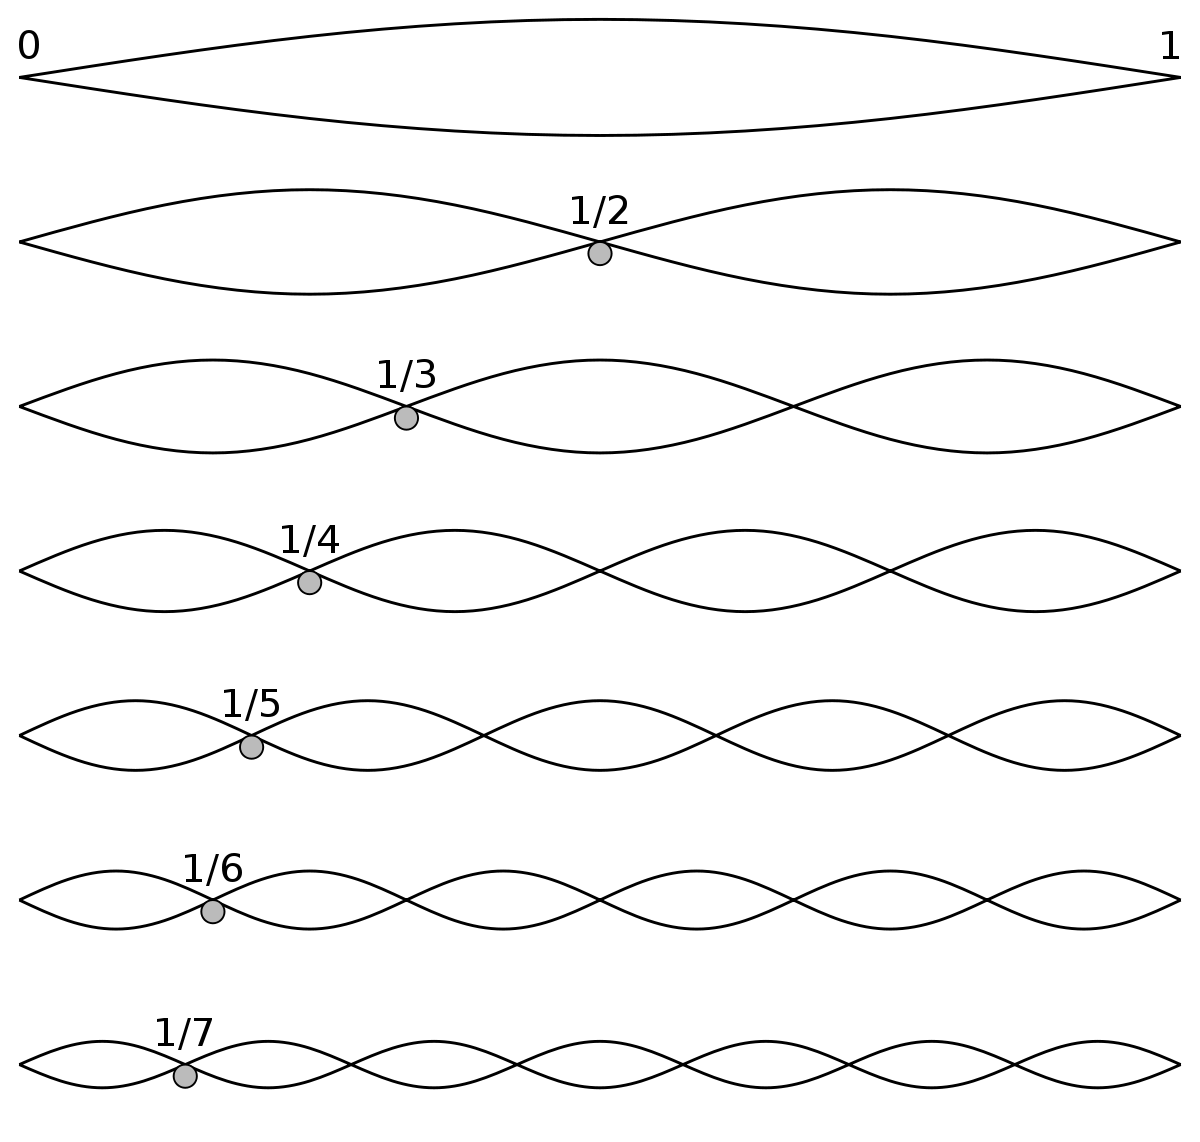
\includegraphics[width=0.5\linewidth]{image/Harmonics.png}
  \caption{A comparison of the wavelengths of waves in a Harmonic Series \autocite{harmonicSeries}.}
\end{figure}

\begin{table}[h!]
  \centering
  \resizebox{0.5\textwidth}{!}{%
    \begin{tabular}{|l|l|l|l|l|l|}
      \hline
      \multicolumn{5}{|l|}{\textbf{Harmonic}} & \textbf{12TET Interval}                                                \\ \hline
      1                                       & 2                       & 4 & 8  & 16 & prime (octave)                 \\ \hline
                                              &                         &   &    & 17 & minor second                   \\ \hline
                                              &                         &   & 9  & 18 & major second                   \\ \hline
                                              &                         &   &    & 19 & minor third                    \\ \hline
                                              &                         & 5 & 10 & 20 & major third                    \\ \hline
                                              &                         &   &    & 21 & fourth                         \\ \hline
                                              &                         &   & 11 & 22 & \multirow{2}{*}{tritone}       \\ \cline{1-5}
                                              &                         &   &    & 23 &                                \\ \hline
                                              & 3                       & 6 & 12 & 24 & fifth                          \\ \hline
                                              &                         &   &    & 25 & \multirow{2}{*}{minor sixth}   \\ \cline{1-5}
                                              &                         &   & 13 & 26 &                                \\ \hline
                                              &                         &   &    & 27 & major sixth                    \\ \hline
                                              &                         & 7 & 14 & 28 & \multirow{2}{*}{minor seventh} \\ \cline{1-5}
                                              &                         &   &    & 29 &                                \\ \hline
                                              &                         &   & 15 & 30 & \multirow{2}{*}{major seventh} \\ \cline{1-5}
                                              &                         &   &    & 31 &                                \\ \hline
    \end{tabular}}
  \caption{The relationship between Harmonic and 12TET intervals.}
  \label{Tab:harmonic_intervals}
\end{table}

Basically, in a roundabout way, we've affirmed a fairly core and commonly known principle of
melody writing: you can almost always resolve to the root. However, this is not the only way in
which interval patterns and the Harmonic series are used to determine consonance. Octaves are
not actually the only case to which the Lipps-Meyers law applies. Melodic intervals can be
simplified the same was fractions can \autocite{intervals}. So then, an interval of 9:6, which
correlate to the major second and major fifth respectively, could also be written as 3:2 and
therefore follows the Lipps-Meyers law.

Another theory on the relationship between harmonics and dissonance was proposed by physicist
Herman von Helmholtz, who posited that the "beats" created by the resonance of two tones which are
close in frequency can help us quantify the dissonance of an interval \autocite{intervals}. Though it is now regarded
that Helmholtz's theory incompletely addresses the nuances of modern physics and music, it is
a valuable discussion because it provides a foundation from a simplified understanding. Because
of its simplicity, we can more clearly view the connections between harmonics and dissonance and
more easily frame it in a way we might be able to apply with computers which also lack such nuance.
An important part of Helmholtz's theory was that harmonic intervals of smaller integers tend to
create higher degrees of consonance \autocite{intervals}. This much is evident in common chord
structures. For example the major tonic is composed of harmonics 1, 3, and 5. Conversely, the
diminished tonic -- commonly viewed as more dissonant -- is composed of the harmonics 1, 11, and 19.

\subsubsection{Contour}

Intervals primarily address each note only in relation to the note directly prior; however, melody
is also constructed upon more macroscopic contexts. This is where contour comes into play. Contour
describes the "shape" of a melody by its repetition, conjunctness, and direction of motion
\autocite{contour}.

Repetition is straightforward; it describes the reoccurrence of a note or series of notes. Too much
repetition in a melody tends to make it feel monotonous, while too little makes it erratic and
difficult to follow \autocite{contour}.

Conjunct motion is also referred to as step-wise motion because it denotes that each note is within
one diatonic step (a major or minor second interval) of the note prior. Its opposite -- disjunct
motion -- refers to melodies containing intervals larger than the diatonic step. Disjunct motion can
add a dynamic element to a melody, but when a melody jumps too large an interval in too short a
time span, it not only generates a lot of tension, it also makes the melody more difficult for a
human to play. For both of these reasons, we should aim to keep our AI outputs to a reduced degree
of disjunctness \autocite{contour}.

Direction in a melody refers specifically to vertical direction. A melody is considered to be
ascending when each note has a higher pitch than the previous and descending when each note is of a
lower pitch than the previous. Fluid motion tends to come across more melodically in music. As
such, it is more desirable to maintain the direction of a melody for a certain period of time
before switching it as opposed to having notes rapidly alternate between ascension and
descension \autocite{contour}.

\subsection{AI}

The artificial intelligence of this project should be able to generate a melody using
a piece of original melody as input. Ideally, it would be able to extend the input at a
similar length and with similar tonality, mood, tension. For this, we research
a couple of different alternatives, with their own sets of advantages, disadvantages, and
trade-offs.

\subsubsection{First Approach: Computer Vision. PixelCNN}

Our original concept for the AI model took a computer vision approach. To begin we would
have had to develop a script which could convert between MIDI data and a PNG
visualization. This image would be similar in structure to what might show on the piano
roll display of a DAW. Each pixel along the vertical axis would represent a key on the
MIDI controller, and each pixel along the horizontal axis would represent some small
fraction of a beat -- hypothetically the length of a sixty-forth note, as this is the
shortest common time interval in music. The hue of each pixel would denote the velocity
of the note being played at that time and pitch - a black pixel would mean no note is
being played while a white pixel would show a note being played at maximum velocity.
These images could then be fed into a Convolutional Neural Network (CNN) which would
replicate the visual patterns and thereby output an image that can be converted back into
a MIDI of a completed melody.

\begin{figure}[h!]
  \centering
  \includegraphics{image/MIDIsample.png}
  \caption{Example of a visualized MIDI file.}
  \label{fig:midi_sample}
\end{figure}

This approach was originally considered for its advantages over a more direct MIDI-based
AI. For starters, when conducting some test trials, it was found that the PNG
visualizations are about a quarter the file size of the original MIDIs they were converted
from. This, in conjunction with the comparatively easy calculations of a CNN on a
simplistic bitmap, suggested that a computer vision model would be fast to train.

Additionally, patterns in music are much easier to recognize through visualization than
through note data. Much of the music theory that determines whether a note is melodic in
context is generalized in that it works according to intervals as opposed to discrete
relationships between specific notes. MIDI files don't provide any information about
scales or chords; they simply list which notes were played. It might take an AI a good bit
of to recognize that the interval between C and E is the same as the interval between F
and A -- and even longer still to determine which intervals are musically dissonant or not,
and in which contexts. When music is visualized, however, it can generalize the same way
it does in abstract theory. Melodic intervals appear visually the same, regardless of the
root note. So rather than having to learn separately that C pairs well with E and F pairs
well with A, it can generalize that any note will pair well with the note that is four
semitones (or in the AI's case, four pixels) above it, known in music theory as the major
third.

The computer vision model was also favored for its level of technical skill. As students,
we have been exposed to the concept of CNNs but have not yet had the opportunity to apply
them. This model felt appropriate for our skill level because it is centered around a
technique we already understand, but it also implements that technique to a degree we have
never attempted before.

\paragraph{PixelCNN}

For the computer vision model, our lead candidate was PixelCNN. Like a standard CNN,
PixelCNN processes its image inputs primarily through layers of masked convolution.
The "masks" used in the convolution layer are square matrices, and each element of the matrix
is a numerical value that denotes the weight of that element. These masks are iterated over the
input image, convolving with the brightness of the pixels under the mask. In colored images,
the process is repeated once for each color channel: red, green, and blue \autocite{pixelCNN}. Depending on the
configuration of the weights in the matrix, different masks can be used to identify different
visual patterns. Each convolution with each mask outputs a two-dimensional array of values
called a feature map.

Unlike a standard CNN, however, PixelCNN specifically uses masks that only allows it to read
one pixel at a time: row by row, and left to right in each row \autocite{pixelCNN}. This enforces that each pixel
is dependent upon only those above and to the left of itself. Using this unique relationship,
PixelCNN has a unique use-case in predicting the bottom half of an image after processing the
top half as input. The AI uses the probability distribution of visual features found in all pixels
iterated through prior to inform the probability distribution it creates to predict the pixels that
will follow \autocite{pixelRNN}.

\begin{figure}[h!]
  \centering
  \includegraphics{image/PixelMask.png}
  \caption{PixelCNN's unique mask prevents the AI from peeking ahead.}
  \label{fig:pixel_mask}
\end{figure}

This made PixelCNN a particularly appropriate candidate for our computer vision model
because completing an image after processing the first half is exactly the mechanic we
planned to use to achieve the melody autofill. All we would have to do is rotate the input
image such that the time axis propagates top to bottom as opposed to left to right.
Additionally, the dependencies that PixelCNN establishes simulate dependencies in music
really well. Whether a note is melodic depends on its context -- specifically, the
notes that came before it in time as well as the other notes being played at the same
time. Adjusting the axes, PixelCNN's dependency upon all pixels above equates to the
current note being dependent on all notes that were played before it. As for its left to
right dependency, chords are typically built upward from the root -- which, when rotated,
would be left to right.

Our main challenge in the use of PixelCNN would be the collection and preprocessing of
training data. For this model to work for our purposes, we would have to convert each MIDI
file into a piano roll visualization which is rotated 90 degrees clockwise.


\subsubsection{Second Approach: Already existent libraries. Magenta.}

Before starting to develop a solution, we checked on existent libraries, academia
research and open source projects. This gave us a broader idea about the possible
factors that can become major challenges such as finding and preparing datasets,
choosing the correct machine learning prediction model, processing hardware
resources, etc.

We found that Google AI has released in 2018 an extensive library for art and music
applications: Magenta Project (\url{https://magenta.tensorflow.org/}).

\begin{figure}[h!]
  \centering
  
\includegraphics[width=\linewidth]{image/fig_JDF01.png}
  \caption{Home Page of Magenta Project From Google AI}
\end{figure}

\paragraph{Magenta Project}

This collection of libraries is specific for music and art (drawing) creation.
For music application, Magenta API contains already trained AI models, tools for MIDI
handling, and datasets that can be directly used to be directly implemented in our
project or being uses as a good standard of reference for benchmark against more
experimental and rudimentary models that can be develop by us.
These collection of libraries are distributed in packages under two main frameworks
and package management system: pip for Python (Magenta) and npm for JavaScript
(Magenta.js). They respectively run on top of the machine learning platform TensorFlow
(https://www.tensorflow.org/) and TensorFlow.js (https://www.tensorflow.org/js).

For this implementation we are designing a full monolithic JavaScript application. For
this reason we will focus on Magenta.js and its machine learning platform,
TensorFlow.js.

Although, Magenta.js is enough to run any of the supported models in the Magenta
project, only the workflow for Python supports the training of new models. This
requires a conversion work between trained models in Python environment and
JavaScript environment. The following section will be dedicated to describe the
supported models for Magenta.js and proposes a workflow to train our own model into
Python environment and generate model checkpoints to be used into JavaScript
environment.

\subsubsection{Magenta Music API}

This API is composed for a set of tools and models to deal with data in MIDI format, that
is of interest for us. Additionally, the API counts with other tools for music
transcription from analog sources of audio that are not considered in the scope of the
present project. Also, this interface provides connection to pre-trained models remotely
hosted that allows some level of training (only for MIDI format) over browser platform,
but this is not considered for our implementation. For the scope of our project, the
following sections of the API can be of special interest: \textbf{OnsetAndFrames} for
translating raw sound to MIDI format, and \textbf{MusicRNN} for melody auto-generation.

\paragraph{OnsetsAndFrames} Described as “model for automatic polyphonic piano music
transcription”(cite: \url{https://magenta.tensorflow.org/onsets-frames}), it is neural
network implementation to translate regular piano sound into MIDI format. In other words,
takes raw piano audio as input and return a MIDI file format with the an equivalent
pattern of digital audio.

\begin{figure}[h!]
  \centering
  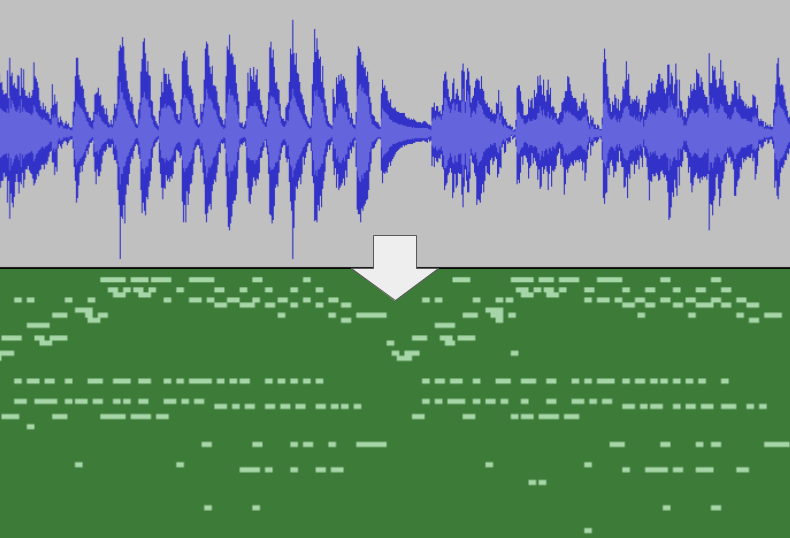
\includegraphics[width=\linewidth]{image/fig_JDF02.png}
  \caption{This model translate raw audio to MIDI format.}
\end{figure}

\paragraph{MusicRNN} Implements a series of recurrent neural networks models based on long
short-time memory language model or LSTM. This is used to predict notes based on long
sequence of related data such is the case of melodies or percussion sets. For this project
we will only consider melody related libraries. In this case, we can find \textbf{MelodyRNN},
\textbf{ImprovRNN} and \textbf{PerformanceRNN}.

\paragraph{MelodyRNN} LSTM implementation that generates melody using an input melody in
MIDI format or generates a random melody without any input priming the model. To achieve
this, the model uses similar techniques applied for natural language analysis. The model
provides four configurations: \textbf{Basic}, \textbf{Mono}, \textbf{Loopback}, and
\textbf{Attention}. Basic can accept as input and produce a baseline melody with a LSTM
model in a reduced MIDI pitch range [48, 84].

\paragraph{Mono} is similar to Basic, but handles full 128 MIDI pitches.

\paragraph{Loopback} handles inputs with added custom labels to allow the model to more easily
recognize patterns that can be periodically repeated across the track on durations of 1 or
2 bars. This decreases the amount of data the model has to store across long sequences of
data.

\paragraph{Attention} is other technique that allows to handle long sequence of data with
a mechanism of encoding-deconding segments of it without having to store the whole data
sequence in coefficients of the RNN. Magenta also provides MusicRNN pre-trained models
under each of the mentioned configuration that can be used as starting point of our
application: \url{basic_rnn}, \url{mono_rnn}, \url{lookback_rnn} and \url{attention_rnn}.

\paragraph{ImprovRNN} This model generate melodies in the same fashion that MelodyRNN, but
incorporates the possibility of giving a progression of chords as input. Then the model
generates melody fitting in the scale of that progression. This is typically done in music
improvisation music execution. This model does not train on MIDI files, but requires the
standard specific format for sharing sheet music files, MusicXML (see Appendix). This
model provides three configurations: \textbf{Basic Improv}, \textbf{Attention Improve},
and \textbf{Chord Pitches Improv}.

\paragraph{Basic Improve} works in the same fashion than Basic MelodyRNN with the addition of
providing a one-hot encoded vector with 48 triad (major, minor, augmented, diminished for
each of the 12 root pitches).

\paragraph{Attention Improve} works similarly to Attention MelodyRNN, providing the same
encoding that the one on Basic Improve.

\paragraph{Chord Pitches Improv} works in the same fashion that Basic Improve but as
output provides a set of three vectors to encode root pitch, absence/presence of pitch
class, and bass pitch class.

\paragraph{PerformanceRNN}: This model intends to simulate the output of a live music
performance. The model provides polyphonic output in PolyphonyRNN format (see Appendix)
with the addition of dynamics and expressing timing. In addition to the parameters present
in PolyphonyRNN format (similar to MIDI) this model also provides parameters representing
note on, note off, time shift and velocity. This model slightly scapes the scope of our
project, but if the implementation is simple enough it could add a nice to have feature
with almost not significant workload.

\paragraph{MusicRNN Python Workflow} Training, Evaluating, Using, and Saving the Model
Although this library provides already pre-trained models, it is also available the option
to train from scratch out own models. This opens the possibilities to generate highly
dedicated models for specific music genre, style, instruments, and similar performance
variables. Of course, on each of those cases, the challenge would be to collect high
volume of data samples for each of the cited cases. However, this can be a good compromise
solution between using an out-of-box solution and developing an entire model from scratch
using a hi-level library such as TensorFlow.

\paragraph{Training Data Processing.} Having a collection of MIDI files in a directory, the
first step is to convert them to NoteSequence buffer protocol (see Appendix). This will
allows the faster and more efficient way to work with data than MIDI files.

\begin{figure}[h!]
  \centering
  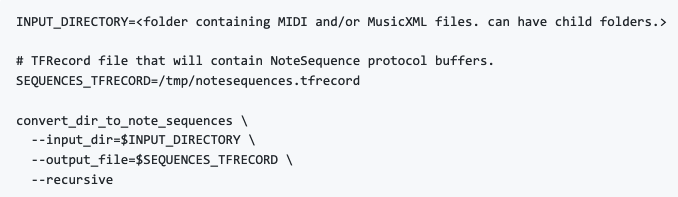
\includegraphics[width=\linewidth]{image/fig_JDF03.png}
  \caption{Example of converting a folder with MIDI files to NoteSequence protocol buffers.}
\end{figure}

%fig_JDF03

The second steps will the creation of SequenceExamples. This is the data format that will
be fed by the model during the fitting stage. The outcome of this part of the process will
be a collection of *.tfrecords files separated into a training collection and evaluation
collection.

\begin{figure}[h!]
  \centering
  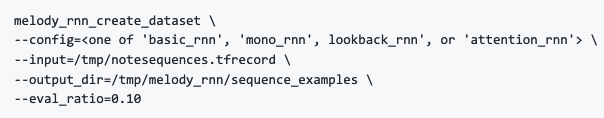
\includegraphics[width=\linewidth]{image/fig_JDF04.png}
  \caption{Example of converting a folder with MIDI files to NoteSequence protocol buffers.}
\end{figure}


For this stage, it is possible to use collections of MIDI files located at

\paragraph{Training the Model.} This stage where the parameters of training are defined
such is the before mentioned configuration of the model, amount of trining cycles, and
data batch size (to limit the usage of memory and prevent out of memory issues training
large models). Also, here is where model hyperparameters are defined such as amount of RNN
layers, previous steps in the data sequence to have into account during the training,
hidden stages, etc.

\begin{figure}[h!]
  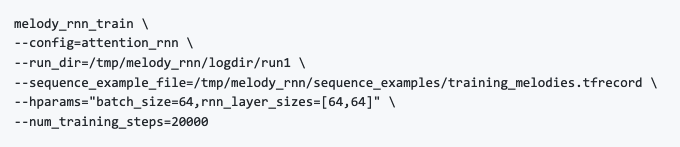
\includegraphics[width=\linewidth]{image/fig_JDF05.png}
  \caption{Example of training model command: \url{melody_rnn_train}}
\end{figure}

It is possible to run evaluation in parallel with the trining to simultaneously measure
the progress in the trining of the model. This is indicated to the framework redirecting
the parameter \url{--sequence_example_file} to a separate set of evaluation data.

\begin{figure}[h!]
  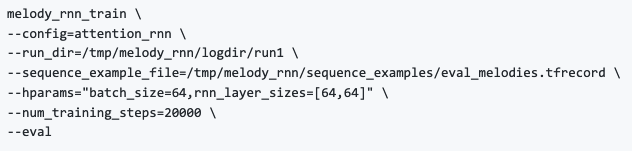
\includegraphics[width=\linewidth]{image/fig_JDF06.png}
  \caption{Example of training model with evaluation in parallel command: —eval}
\end{figure}


To be able to visualize the progress of the training and evaluation of the model, it is
possible to run the log command and access to the local host (\url{http://localhost:6006})
with any browser.

\begin{figure}[h!]
  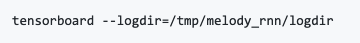
\includegraphics[width=\linewidth]{image/fig_JDF07.png}
  \caption{Command to activate the log register (tensorboard) during train evaluation
    cycles.}
\end{figure}



\paragraph{Generating Melodies with Trained Model.} During or after the training, it is
possible to run the model and generate melodies with the latest generated coefficients or
\url{checkpoint}. For this is the \url{—run_dir} parameters will point to the location
where of the trining job, containing in a subdirectory within that location the most
recent checkpoint file. All other parameters used to run the melody generation should be
the same as in the training command in execution (if the model will be executed before the
training ends). Also is needed to specify the output directory where all the generated
melodies will be placed. To start the generation of the melody, at least one note is
required as seed.

\begin{figure}[h!]
  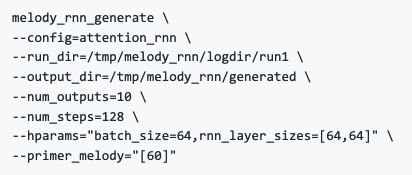
\includegraphics[width=\linewidth]{image/fig_JDF08.png}
  \caption{Command to generate a melody using a single note C4 in the \url{—primer_melody} parameter}
\end{figure}


\paragraph{Saving the Trained Model.} Magenta uses as output bundle format that can be
produced with a single command, grouping all the data that will be required for reusing
the model such as model checkpoint, metagraph (the information about the conection
between neurons), and other metadata that will be required to reconstruct the model
afterwards.

\begin{figure}[h!]
  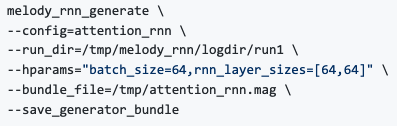
\includegraphics[width=\linewidth]{image/fig_JDF09.png}
  \caption{Command to generate a bundle file with the information of the model: \url{—save_generator_bundle}}
\end{figure}

\paragraph{Converting Python Trained Models to TensorFlow.js.} In order to work in a JavaScript
environment, it is required to convert the bundle format or any of the TensorFlow/Keras
format into TensorFlow.js format. For this, it will be used \url{tensorflowjs_converter}
command in the following fashion:

\begin{figure}[h!]
  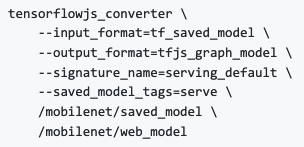
\includegraphics[width=\linewidth]{image/fig_JDF10.png}
  \caption{Command to convert TensorFlow SavedModel into TensorFlow.js comptible format}
\end{figure}

\subsubsection{Third Approach: Develop our own RNN. LSTM.}

On our first approach in section 5.3.1, the data was planned to be treated as a spacial
2D disposition as is in a picture. For this reason, the solution was planned to be
execute with convolutional neural networks to be able to parse the patterns on visual
representation of small segments of melodies. This approach can be impractical if
there is intention to process long sequence of ordered data such is music.

As we seen in section 5.3.2, the most common model is based on recurrent neural
networks. These kind of models were developed with the idea of processing sequential
data that follows patterns and relations across long distances between different point
in the sequence. Regular neural network cannot register these kind of patterns (see
Regular Neural Networks Appendix). This feeding forward patter to process data is
what gives the character of ‘recurrent’ to these models.

A similar to music sequential interrelated pattern of data, but more complex case is the
analysis of natural language. From this field is that many of these ideas are applied to
music processing and modeling. This section will explain how those ideas were
developed, and how that can be translated to music melody prediction. Also, we will
explore TensorFlow API as our framework to develop for this approach.

\paragraph{Autoregressive Model, RNN and LSTM.} Music is composed for a finite amount of
combinations that follows structures such as harmony. As already was explained, these is
based on concept as scales, progressions, and interval. For this reason, it is expected
that for a determined sequence, there will be a distribution of probabilities function
that describe what key will be the next one in the melody. Basically, we are calculating
conditional probabilities related to already seen segment of data. In other words, the
possibility that the following key in the melody, with be proportional to a determined
preceded sequence:

\begin{equation}
  x_t \sim P \left( x_t \vert  x_{t - 1}, ..., x_1 \right)
\end{equation}

In order to capture these relations and probabilities, we can use a model that store
probabilities coefficients of each possible sequence. These coefficients can be used to
calculate the probability of the pitch at time ’t’ using the already known pitch at time
’t-1’. If this is done recurrently, we are in presence of a autoregressive model. The
coefficients used to calculate the prediction are never ‘seen’ and they are constantly
being updated during training stage, for this reason they are called ‘hidden states’.

\begin{figure}[h!]
  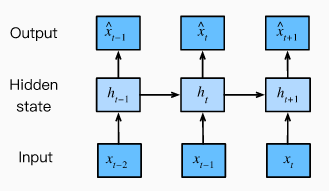
\includegraphics[width=\linewidth]{image/fig_JDF12.png}
  \caption{Latent Autoregressive Model}
\end{figure}


Still, this basic model has some issues: the storage overhead of the model for hidden
stage can be unmanageable (imagine saving all possible combination of keys with not
length limitation). Also, this model can perform well in producing interpolation of known
data. On the contrary, experimental results shows that errors add-up and the model
perform poorly or directly does not perform at all after relatively few predictions outside
the known sequence. As an experimental example, the prediction of values of a
function start performing after 4-steps ahead, to finally converging to constant values
in just 64-steps predictions:

\begin{figure}[h!]
  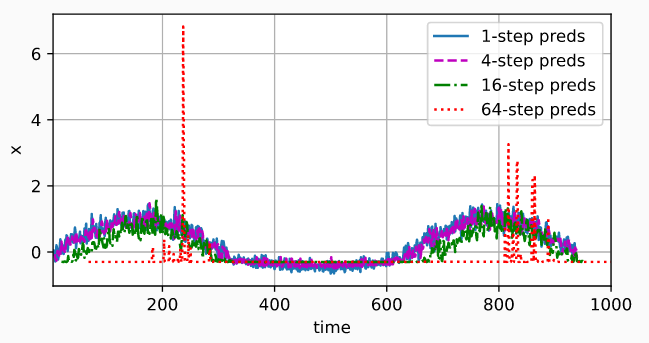
\includegraphics[width=\linewidth]{image/fig_JDF13.png}
  \caption{Experiment of Latent Autoregressive Model Prediction}
\end{figure}


This issue known is product of gradient explosion or vanishing. The first case is when
the network coefficients diverges to infinity, not producing any learning effect on the
network. The gradient vanishing occurs when the coefficients converges to zero and
the training back propagation information is lost. This problem is common in common
front-feeding/back-propagation RNN.

To avoid vanishing, it is necessary to implement a network that can maintain the
training information long back to the structure of the network. In other words, there
should be an implementation that allows the flow the intact gradient information not
only to the latest layer in the network, but also to some hidden layers in across the
structure to be able to learn from this information. This is the motivation behind the
creation of long short-term memory (LSTM) networks.

LSMT introduces a new type of neural network architecture unit: the LSMT cell.

\begin{figure}[h!]
  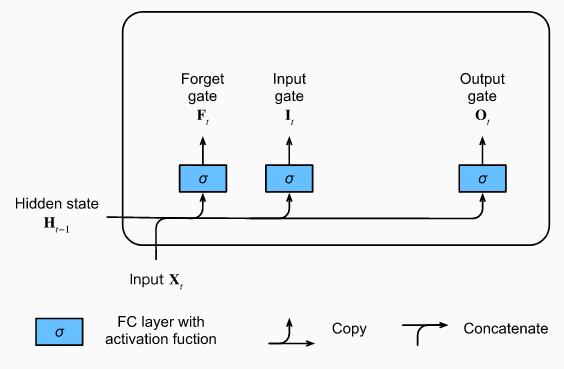
\includegraphics[width=\linewidth]{image/fig_JDF14.png}
  \caption{Experiment of Latent Autoregressive Model Prediction}
\end{figure}


This structure operates as a gate using as input the current data state and the hidden
state from the before step in the network. From these inputs the cell takes state of
modifying its own hidden state or keep it unmodified to be fed to the next cell.

\paragraph{Data Gather and Processing} Before diving into the implementation of a model
using LSTM cells, we need to gather and process data in a compatible format for our
machine learning framework.

For the gathering of large collection of data, it is possible to use large MIDI collection
like the one located at https://www.mutopiaproject.org/.

\begin{figure}[h!]
  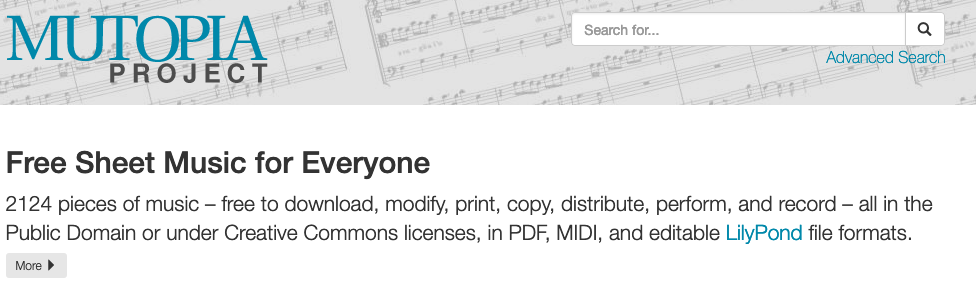
\includegraphics[width=\linewidth]{image/fig_JDF15.png}
  \caption{Mutopia Project contains large free-to-use collection of music in MIDI format }
\end{figure}


Because the website does not support batch download collection, we would need to implement
a script for ‘web scrapping’ a large quantity of these files. This can be done without
major challenges using a Python implementation as follow:

\begin{figure}[h!]
  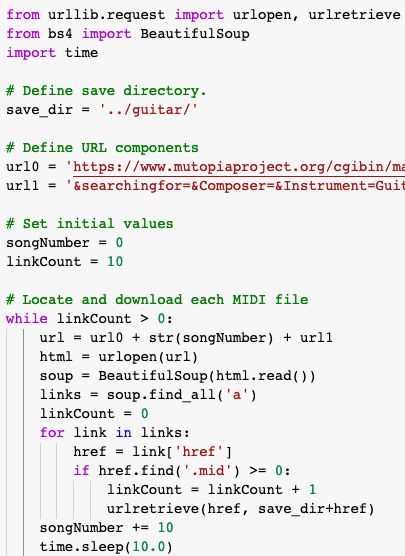
\includegraphics[width=\linewidth]{image/fig_JDF16.png}
  \caption{Example of web scraping code for data collection }
\end{figure}


After the collection of the data, we need to process it to be used for training and
evaluation. Knowing that Tensorflow model layer requires a vectorial representation of
inputs, we need put in place a workflow to convert MIDI files into compatible vectors that
represents a melody to be fed to the model.

To process the MIDI collection, it is possible to use a library ‘music21’
(https://web.mit.edu/music21/). The representation, as already explained, consist in the
note and duration of each note. For this particular conversion, the classes required are:
converter, pitch, and interval. Later, we can loop through all the MIDI files located in a
single directory with a code as follows:

\begin{figure}[h!]
  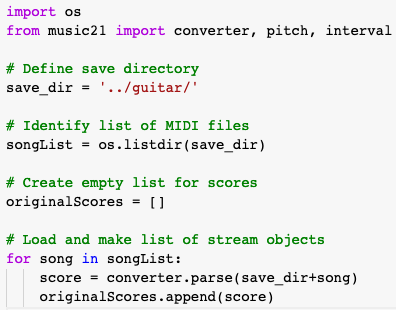
\includegraphics[width=\linewidth]{image/fig_JDF17.png}
  \caption{Example of converting from MIDI to scores from local directory }
\end{figure}


Still there is an issue with this data set: many of the MIDI files contains polyphonic
song (many instruments). This could be resource intensive and also is probable to add a
significant amount of noise in the data set, producing undesirable predictions. For this
reason it is needed to convert any polyphonic MIDI to a monophonic format, extracting the
main melody in a single instrument. That can be done by the next function:

\begin{figure}[h!]
  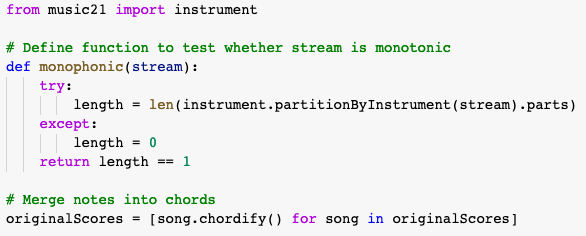
\includegraphics[width=\linewidth]{image/fig_JDF18.png}
  \caption{Example of converting from polyphonic score to monophonic }
\end{figure}


Finally, all the converted score are possible to convert to three separate lists: notes,
chords, and duration. This is an example of this processing code:

\begin{figure}[h!]
  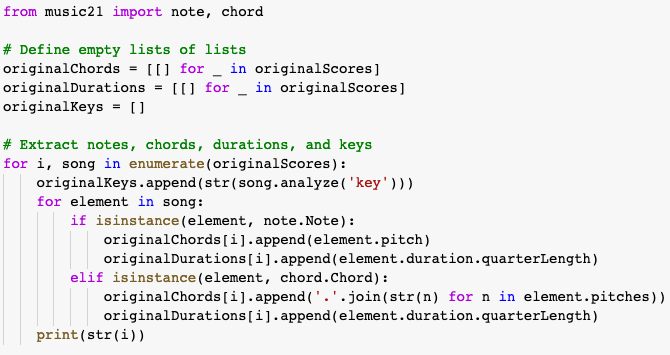
\includegraphics[width=\linewidth]{image/fig_JDF19.png}
  \caption{Code to place in lists notes, chords and duration }
\end{figure}


Some feature engineering can be done to reduce the amount of data is processed by the
model, such as using just MIDI compositions executed in a specific instrument,
compositions of single author, transposition of all songs to a single set of keys, etc.
Also, it is possible to filter out identical sequences to decrease the chances of faster
overfitting of the model. This will be researched during the execution of this project.

The last step on the preparation of the data will be the separation of the converted
melodies into stream of equal length sequences. An example of the code to perform this
action to a dataset that was transposed to C major key as part of feature reduction
follows like:

\begin{figure}[h!]
  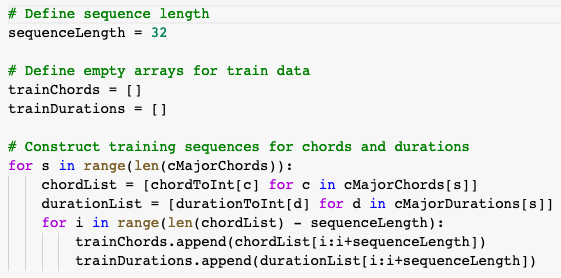
\includegraphics[width=\linewidth]{image/fig_JDF20.png}
  \caption{Code used to segment the data in equal length. In this case 32 keys.}
\end{figure}

Additionally, it will be needed to serialize all these streams into a file format to be
able to be retrieved later. This can be series of CSV files or some kind of buffer stream
as the one mentioned in the before section.


\paragraph{Implementation of LSTM with TensorFlow.} The implementation from scratch of a deep learning
model can be daunting. The amount of possibilities are endless, and without a clear path
to follow, but the moto “start simple and build-up from there”. For this reason, as
starting point, we could use an existent architecture that is already tested and
published. For illustrating the case in the current documentation, we will describe the
architecture used at this location:

\begin{figure}[h!]
  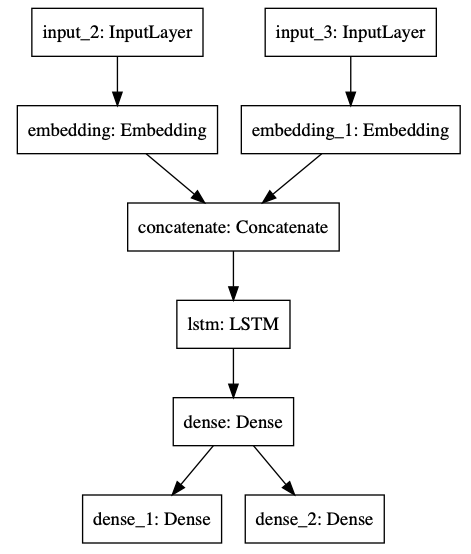
\includegraphics[width=\linewidth]{image/fig_JDF21.png}
  \caption{Possible architecture to be implemented as starting point for our LSTM RNN }
\end{figure}


This architecture posses two inputs: chord input and duration input. The network should be
able to train both parameters in parallel. Also, for the same reason, it will be needed
two outputs for predicting exactly those same parameters.

After each input, and embedding layer will be sequentially connected. This will transform
each chord and duration to a compact format that allocate similar values to similar keys
instead of a large one-hot encoded format with 64 elements where except for one all others
are zero.

The compact chord representation on one side, and the duration representation on the
other, will be concatenated in a single input. This step will keep the association of each
chord and duration placing them in a single data structures ready to be processed by the
core layer of this data structure: the LSTM cell layer.

The LSTM layer will be keep register of hidden coefficients that holds the information
about the probabilities of the concatenated input sequences primed during the training
stages.

Finally, the set of dense layer should increase density of representative states of the
network for all the different patterns: first chord and duration concatenated, and later
in separate way to be processed by a softmax activation function that returns the
probability of the prediction in the output layer.

\begin{figure}[h!]
  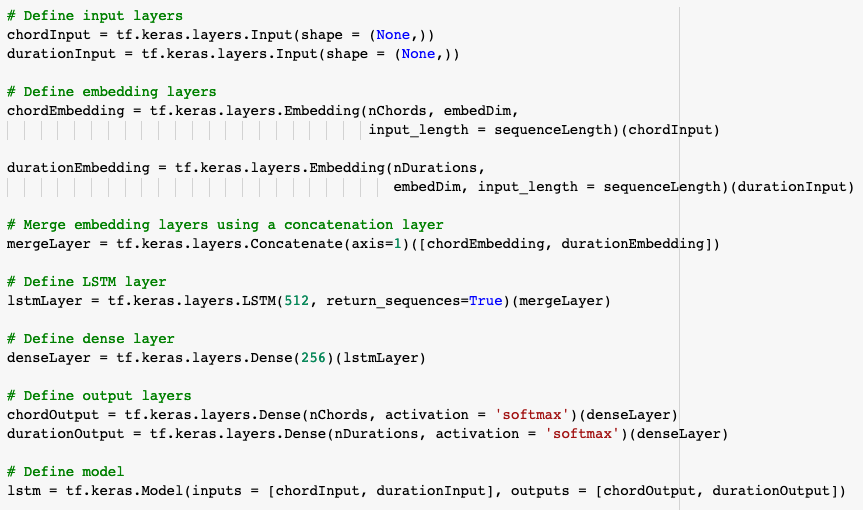
\includegraphics[width=\linewidth]{image/fig_JDF22.png}
  \caption{Example of the code to implement a double input, double output LSTM RNN }
\end{figure}


\paragraph{Training of the Model.} After the completed the architecture of the network, it is possible
to start compilation and training of the model. For this case, it is required to define a
loss function and optimizer technique, the will track the minimization of the loss. The
training step can be initialized defining the size of the training batch and the amount of
epochs (training iterations). An example of the code that implements these two steps as
follows:

\begin{figure}[h!]
  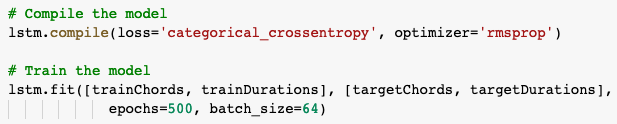
\includegraphics[width=\linewidth]{image/fig_JDF23.png}
  \caption{Example of compilation and training of Tensorflow LSTM RNN }
\end{figure}

\paragraph{Using Model to Generate Melody.}
Once the training is done, it is possible to feed the model with a sequence of notes and
generate melody based on the input. This process can be done iteratively, in other words,
the predicted output can be used again as input to generate a new output that will be
concatenated at the end of the already existent piece of melody, repeating this stage
indefinitely for as long as desired. As example of this implementation, the following code
uses a 32 chord sequence as initial input, and generate 100 segments of equal size as
output:

\begin{figure}[h!]
  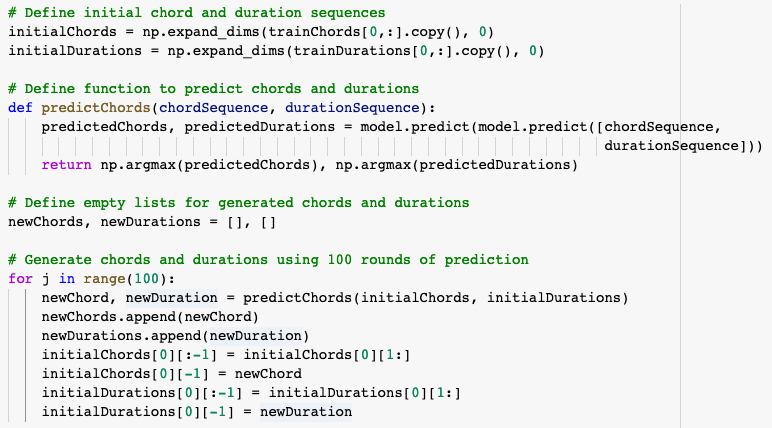
\includegraphics[width=\linewidth]{image/fig_JDF24.png}
  \caption{Example of newly generate melody with model }
\end{figure}

This step will generate the melody in the format that was parsed the MIDI file for
training and input. Still it is required to convert it back to MIDI to be able to
reproduce it.

\paragraph{Reconstructing MIDI File From Generated Melody.} This step is very similar to the one
already described to parse MIDI into lists to use as data set for TensorFlow model. This
is simply the reversion of that steps. For this, it is used again the music21 library as
follows:

\begin{figure}[h!]
  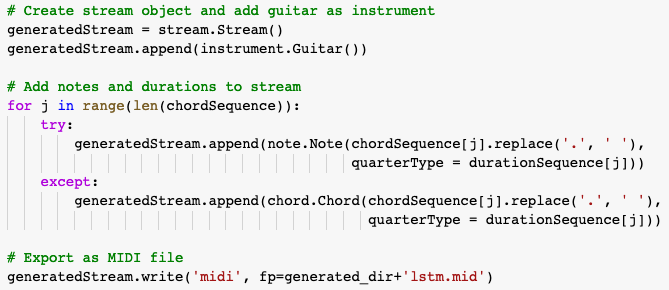
\includegraphics[width=\linewidth]{image/fig_JDF25.png}
  \caption{Example of constructing a new MIDI file with the prediction generated}
\end{figure}


\paragraph{Model Reuse and Conversion to JavaScript Platform.} As already mentioned in the
before section, to be able to use the trained model into a monolithic JavaScript
environment, it is required to convert the network weights into a TensorFlow.js compatible
format.

In this case, a possible export format for weights can be ‘*.hdf5’. To implement saving
the best model found during training we need to modify the call of the fit method on the
model on the training section. As a side note, this workflow defines as ‘the best trained
model’ as the one with the lowest loss validation value during the training iterations.

After training, testing and evaluating the model generated, the weights are exported to
JavaScript compatible format in the following way:

This project will count with unit testing at all possible point in the code. For this,
before proceeding to a random generation of a model, that will not produce deterministic
results, a seed value for random generation will be provide.

The main focus of unit test would be around functions that provides a result using
principally code written by our team. There are sections of code related to the pipeline
of TensorFlow/Keras framework that we trust is largely test as part of those libraries.

As dataset for this stage a collection of well known melody sequence will be used for
benchmark.

\begin{figure}[h!]
  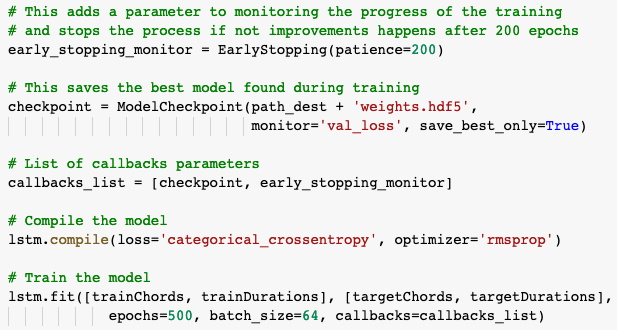
\includegraphics[width=\linewidth]{image/fig_JDF26.png}
  \caption{Addition of monitoring parameters to save the best model}
\end{figure}

\subsection{Embedded Controller Comparisons}
\label{sec:embedded_controllers}

\subsubsection{Raspberry Pi 4 Model B}

\begin{figure}[h!]
  \centering
  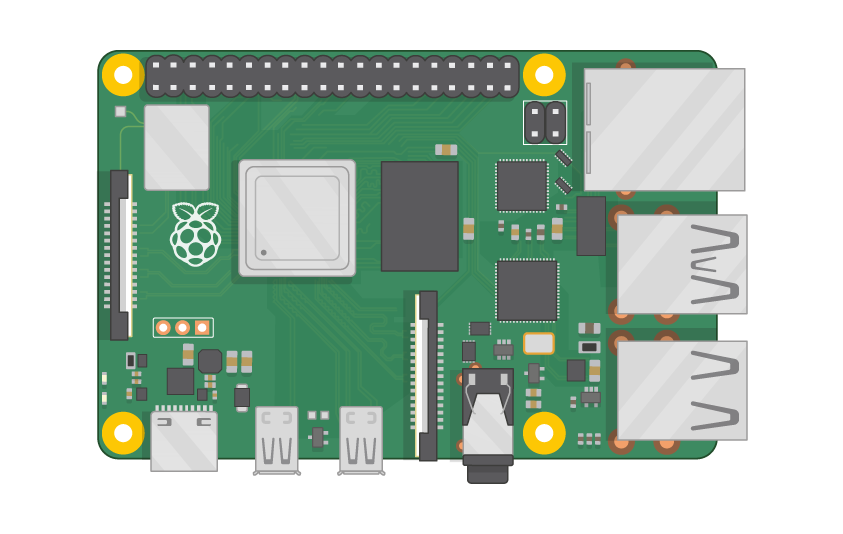
\includegraphics[width=\linewidth]{image/raspberry-pi.png}
  \caption{The Raspberry Pi 4B \autocite{raspberry-pi-4b}.}
  \label{fig:rpi4b}
\end{figure}

The Raspberry Pi is a mini-computer which can act as an embedded controller using GPIO
pins. This is an appealing option to us, as it is easy to use and members of our group
have previous experience with it, and one of our members already owning a Raspberry Pi to
test on. What makes the Raspberry Pi more than just an embedded controller is the GPIO
pins that are located in the top of the board as seen in \autoref{fig:rpi4b}. These pins
are designed to allow the Pi to interface with other electronics, such as buttons attached
to our keys. Each pin serve a different purpose, and we will be using a few of them.
Otherwise, the Raspberry Pi 4 functions as a normal computer, with the ability to plug in
a keyboard, mouse and monitor. The Raspberry Pi can run any armv7 Linux distro. The
operating system is loaded onto it using an SD card. The Raspberry Pi is typically powered
using USB-C and a power supply, but it can also be powered through one of the GPIO ports,
with a 5V connection. The Raspberry Pi also features an ethernet port and a headphone
jack.

The Raspberry Pi has a baseline cost of \$35 for the 2 GB of RAM edition, \$55 for the 4
GB edition, and \$75 for the 8 GB edition. We intend to use the 4 GB edition, which will
meet our memory requirements for running an electron app and an AI. This price is within
our budget constraints.

The Raspberry Pi can be seen as overkill for many projects, where a cheaper embedded
controller, such as an Adruino, could be used instead. Our project is computationally
expensive, so it makes sense for us to use good hardware. Although it may be possible to
do this project with a cheaper embedded controller, it would be risky to design our
prototype with cheaper hardware. We know from preliminary testing that the Raspberry Pi
will provide the computation power and memory our project needs. We prefer to start with
hardware we know will meet our specifications from the start.

\subsubsection{Conclusion}

We have decided to use the Raspberry Pi 4 for our project. From our research , we know
that the Raspberry Pi will meet our specifications. Our previous experience with Raspberry
Pi is a big advantage, and working with a full-blown Linux environment will save us
valuable development time.


\subsection{DAW Frontend Technologies}

We are looking to use a browser-based frontend Design. This approach is ideal for its ease
of implementing a user interface as well as its cross-platform compatibility. Should we
decide to make the software even more portable by isolating it from the MIDI controller,
it will be viewable on any device that can run a browser. And because of the computational
limits of the MIDI controller, any modern device that is suited for a browser will
inherently be able to run the MIDI autofill software as well.

We experimented with several options for a UI-building environment. Our first consideration was
React, a JavaScript library for app development. One of the appealing features of React was that
not only do the programs operate on an object-oriented basis, but the functionality of the
application shell is also very object-oriented. This makes more flexible functionality simpler to
achieve. For example, the render function allows the programmer to merge HTML and JS elements so
they can add reactivity to the markup elements without having to repeatedly alter the properties
in JS code.

However, its major downside is that as a new library, it implements a lot of functions and
techniques our team are not familiar with in the core functionality of the program. While it would
be possible to come to understand these concepts through trial and reading documentation, as
mentioned in \textbf{\ref{sec:constraints} \nameref{sec:constraints}}, our choices are motivated by
what is achievable on a strict timeline. For a project as complex as we plan to develop, it would
be better to use a tool we have better mastery with.

Our second consideration was Electron, a desktop app development API that’s based on website-style
design. As many of our team members have encountered projects involving web development, this
option was much more viable to learn at a proficient level. For the most part, the website
functionality remains the same, but porting it into an Electron shell converts it into an
application.

Another strong candidate was Google’s Flutter. Flutter’s default stylization is sleek and fits in
well with the modern aesthetic of technology. Plus, its widgets allow for more polish on a UI that
also has more niche functionality. Our frontrunners after all options had been proposed were
Electron and Flutter, but ultimately it was our hardware constraints that pointed us toward
Electron because the HTML and JavaScript application was the most likely to be compatible to run on
the Raspberry Pi.

As established in \textbf{\ref{sec:daw} \nameref{sec:daw}}, the primary aspect of the UI
will be the piano roll display. The frontend will be responsible for reading the MIDI
messages and converting the note ON/OFF and timing clock features into the position and
dimensions of an arbitrary number of UI elements -- each representing a note which can be
edited.

\subsection{Raspberry Pi}

As mentioned in \textbf{\ref{sec:embedded_controllers} \nameref{sec:embedded_controllers}},
the Raspberry Pi is mini-computer which can also function as an embedded controller. The
model we're interested in is the Raspberry Pi 4B, which is the latest model and has the
best hardware. After an analysis of other solutions, we have decided that the
Raspberry Pi is the best fit for our project. To that end, we have researched how the
Raspberry Pi can be configured for use in our project.

\subsubsection{Operating System Choice}

The first configuration choice that needs to be made is the operating system. A Raspberry
Pi out of the box has no operating system. An image must be flashed to an SD card to make
the Raspberry Pi useful. Raspberry Pi's typically run some form of Linux. The Raspberry Pi
4B model uses the AArch64 architecture. It can run most AArch64 based Linux distros, but
we must limit ourselves to armv7 (32 bit) operating systems, as tensorflow does not
natively support AArch64 as of the time of writing. Tensorflow lite supports AArch64, but
tensorflow-lite has a limited number of supported operations, which can inhibit our
development. There are still many OS choices available, as there are many flavors of Linux
that can run on the armv7 architecture. Some common choices for Raspberry Pi include
Raspberry Pi OS (formerly known as Raspian), Arch Linux ARM, and DietPi. Each OS has its
advantages and drawbacks, and it is important for us to select a distro that is well
suited for our use case. We will need to modify the system heavily for our purposes, but
we need a good baseline for modification.

We need our distro to be a lightweight bootloader for our application. There are many
examples of highly specialized distros designed for one specific task. Examples
include RetroPIE, which is used to run retro video games, or OpenMediaVault, which is used
to turn the device into a networked storage device. This is similar to what we want our
operating system to do. Our use case for the Raspberry Pi is to run one specialized
application that we ourselves develop. It should boot straight into our application with
no other UI from the operating system. The best solution for us is to have a custom distro
just for running our application. Developing a Linux distro from scratch is a difficult
process that is out of the scope of this project. But what we can do is modify an existing
distro to suite our needs. We plan to do this process using a tool called Packer,
described in more detail in Section \ref{sec:packer}.

\paragraph{Raspberry Pi OS}

\begin{figure}[h!]
  \centering
  \includegraphics[width=\linewidth]{image/rpi-desktop.png}
  \caption{The Raspberry PI OS Desktop \autocite{rpi-desktop}.}
  \label{fig:rpios}
\end{figure}

The most common operating system used for Raspberry Pi is Raspberry Pi OS, which is
developed by the Raspberry Pi Foundation. This is a specially tailored version of Debian
for the Raspberry Pi. This is a common choice for any general purpose usage the Pi. It can
be used like a normal desktop computer when a mouse, keyboard, and monitor are plugged in.
This is a "batteries included" distro that includes things we do not need, such as a
desktop environment, login manager, and various desktop apps. The extra software from this
distro can hinder performance and waste SD card space.

Raspberry Pi Foundation is aware that this distro is too heavy for many Raspberry Pi
projects. To mitigate this issue, they provide lightweight edition known as Raspberry Pi
OS Lite. This version does not include any desktop environment or other extraneous
software. As a result, Raspberry Pi OS Lite fits in 442 MB, which is a big improvement
over Raspberry Pi OS, which is 1175 MB. This makes Raspberry Pi OS Lite a better choice
for our use case, as it would be easier for us to build up to what we need rather than to
cut what we do not need.

\subparagraph{Pros}
\begin{itemize}
  \item Very well documented
  \item Has the best support for Raspberry Pi
\end{itemize}

\subparagraph{Cons}
\begin{itemize}
  \item Comes with unnecessary software
\end{itemize}

\paragraph{DietPI}

DietPi is like Raspberry Pi OS Lite in that it is a lightweight distro. DietPi's claims to
be even lighter than Raspberry Pi OS Lite. It occupies 589 Mb on the SD card, while
Raspberry Pi OS occupies 1424 MB. There are other system optimizations in place to improve
general performance as well. After boot, there are 11 total processes, versus 18 total
processes running on Raspberry Pi OS. This is a good choice for base system. It is easier
for us to start lightweight and add what we need, rather than to start with a bloated
system and strip it down. DietPi comes with a flexible configuration utility that allows
the system to be customized for a specific use case, as show in \autoref{fig:dietpi}.

DietPi includes a configuration menu in the installation for software that runs after
boot. In this menu there is a way to run chromium in kiosk mode. This is an item that we
need to configured anyways, as described in Section \ref{sec:research:subsec:os_config},
which also makes DietPi an appealing choice. DietPi also supports a fully automated
installation process, which we intend to take advantage of, as will save us time from
needing to flash the Raspberry Pi and go through the installation process whenever we
change the operating system configuration.

The main downside to using DietPI over Raspberry PI OS is that there are many tutorials
and documentation for using the Raspberry PI with Raspberry PI OS, that may not apply to
using DietPI, or will be a different process.

\subparagraph{Pros}
\begin{itemize}
  \item Lightweight
  \item Automated installation
  \item Flexible and easy configuration
\end{itemize}

\subparagraph{Cons}
\begin{itemize}
  \item Not as much documentation as Raspberry Pi OS
\end{itemize}

\begin{figure}[h!]
  \centering
  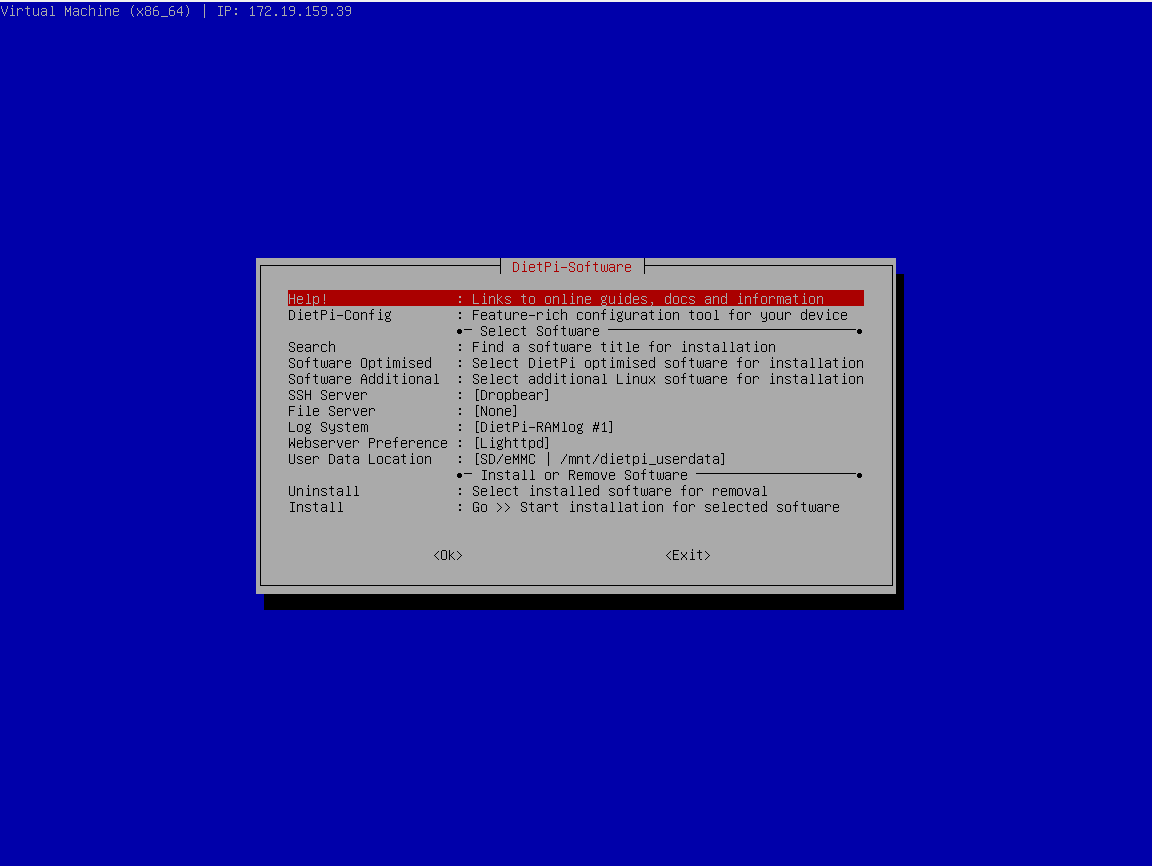
\includegraphics[width=\linewidth]{image/dietpi-config.png}
  \caption{DietPi's Installation Menu.}
  \label{fig:dietpi}
\end{figure}

\paragraph{Conclusion}

From our research, we have decided to use DietPi as a baseline operating system for our
project. The lightweight aspect suits us well, as we only need to boot a single
application. The high degree of customization makes it easy to have a minimal system
tailored to our application. The easy chromium kiosk mode configuration is also a big
bonus, as it relieves us from a configuration burden. The installation of DietPi will be
automated using the automated install process, and further customized using Packer.

\subsubsection{Operating System Installation}

\begin{figure}[h!]
  \centering
  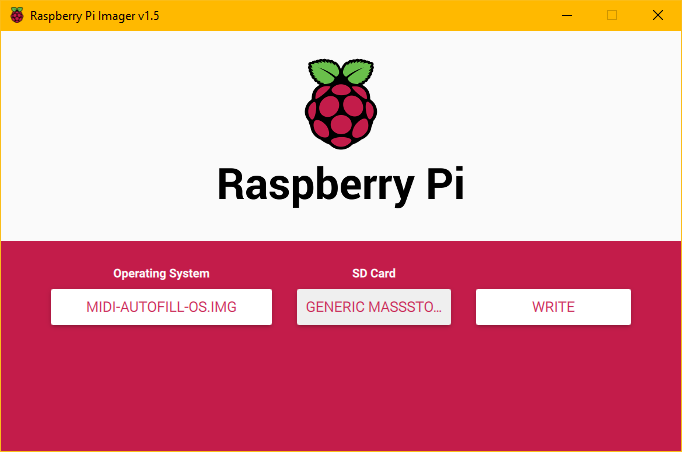
\includegraphics[width=\linewidth]{image/rpi-imager.png}
  \caption{The Raspberry Pi Imager Utility.}
  \label{fig:rpi-imager}
\end{figure}

Installing the OS to the Raspberry PI is a simple process. The operating system is
provided from the DietPi website as a \url{.iso} file. An \url{.iso} file is a
representation of a disk archive in a file. In our case, we will be using a modified
\url{.img} file from Packer, but the usage is exactly the same. This image from Packer can
be flashed to an SD card using the Raspberry Pi Imaging utility (See
\autoref{fig:rpi-imager}). We use a USB SD card reader for this purpose. Once the SD card
is flashed, it can be inserted into the Raspberry Pi. Now, once the Raspberry Pi is
powered on, the device will boot straight into the operating system. Typically, this would
be followed with a lengthy installation process, but we have already automated the install
onto the image ahead of time using Packer and the DietPI installation automation process.

\subsubsection{Operating System Configuration}
\label{sec:research:subsec:os_config}

The operating system will need to be configured for our use-case. We need to get the
operating system to boot a single GUI application, our DAW, without displaying any other
UI from the desktop environment (DE). There may be more applications separate from the DAW
that will run in the background which also must started immediately after boot such as an
application that acts as the MIDI backend, sending the MIDI notes to the host PC, which
will likely be a separate component from the DAW itself. The operating system will need to
be configured to not permit any networking out of security and privacy concerns.

To only display a single application, we need to configure the graphics system in our
distro. Graphics in Linux are done through the X Window System. In modern apps, X is
mostly agnostic to the UI, and is used for providing UI toolkits a method for accessing
bitmaps to windows. X can be configured in a variety of ways. The way we intend to
configure X is to host a single fullscreen application for our DAW. This can be done
through the \url{.xinitrc} file. This file specifies which commands to run whenever the X
server starts. By including the command to run our application in there, we will have a
single window at startup.

\begin{lstlisting}[language=bash, label={lst:xinitrc}, caption=Example .xinitrc]
#!/bin/sh

exec chromium --kiosk http://127.0.0.1:8080/
\end{lstlisting}

Because our app is browser based, the startup application will be a web browser. In our
case we want to use the Chromium browser, which is the open source variant of Google
Chrome. Chromium has a feature called Kiosk mode, which puts the browser in fullscreen
with no border or frame \autocite{chromiumKioskMode}. This in combination with the xinitrc
file fulfills our requirement of only having a single fullscreen application with no other
UI. This feature can be enabled through the \url{--kiosk} command line flag
\autocite{chromiumKioskMode}. See \nameref{lst:xinitrc} for an example of an xinitrc that
launches chromium in fullscreen mode. DietPi can also handle this configuration for us,
using the \url{dietpi-autostart} configuration utility (See
\autoref{fig:dietpi-autostart}).

\begin{figure}[h!]
  \centering
  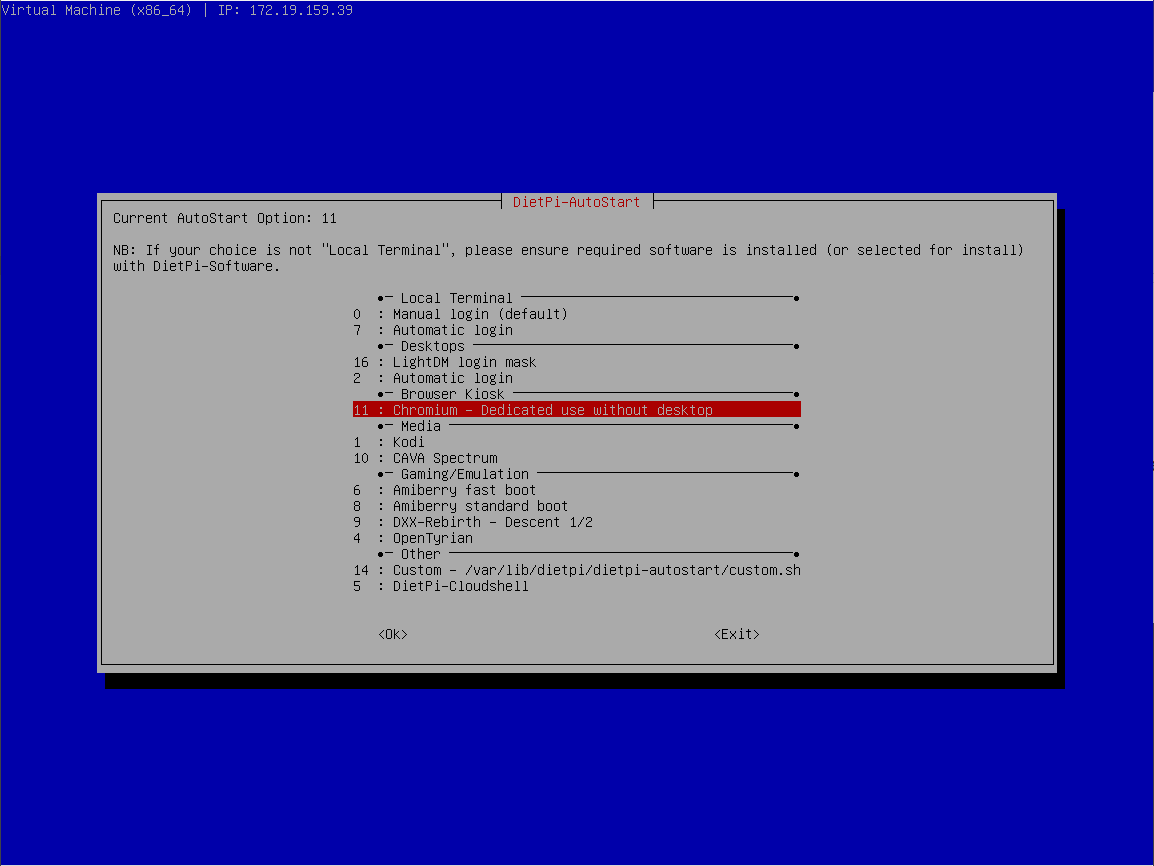
\includegraphics[width=\linewidth]{image/dietpi-autostart.png}
  \caption{DietPi's Autostart Menu with Chromium Kiosk Option.}
  \label{fig:dietpi-autostart}
\end{figure}

For the final product, we will want to have networking disabled. We will need network
connectivity while in development, so we can use SSH and LAN, so we need to make sure that
we switch it off for the final rpdouct. Networking can disabled through the
\url{/etc/network/interfaces} config file. This config file is used to declare all
networking interfaces, and the interfaces can be removed by simply removing all lines
declaring a networking interface in that file. We can remove all networking interfaces
except for the loopback (\url{lo}) interface, which is the localhost interface that is
important for the system to function properly.

The MIDI connection is going to happen through MIDI over Bluetooth Low Energy, which will
require operating system configuration. This configuration happens through the BlueZ
stack, which is the Linux component responsible for handling Bluetooth, and will be
configured using the BlueZ utilities and configuration files. This configuration process
is quite extensive and is covered in more detail in \nameref{sec:ble_midi}.

\subsubsection{Packer}
\label{sec:packer}

A solution we found for customizing an existing Linux distro is Packer. Packer is a
utility that can take an existing operating system image, change it, and produce a new
image. Modification is done through provisioners, which exist to perform steps, such as
copying files, running shell commands, setting permissions, etc. Packer relies on builders
to carry out the tasks laid out in a configuration file. The builder we will use is called
packer-builder-arm, which builds ARM images and is suitable for a Raspberry Pi.

Packer is configured through simple JSON files. These JSON files contain information about
the original operating system's image, such as the URL it's hosted on, as well as other
metadata about the image. The JSON file also configures provisioners to modify the
operating system. With these provisioners, we can create our own packer json config file to
setup all the tasks described in \nameref{sec:research:subsec:os_config}.

One of the provisioners we will use is the file provisioner, which copies files from the
build tree over to the operating system. For example, the file provisioner can copy the
\url{.xinitrc} file to the home directory, which configures X11 for our application.
We will also use file provisioners to copy over the \url{/boot/} modifications required to
turn the device into a USB gadget, as described in Section \ref{sec:midi_peripheral}.

We will use shell provisioners to run all the DietPi installation and configuration steps.
This will include automating the options we specify in the \url{dietpi-config} and
\url{dietpi-software} utilities. We will also use shell provisioners to clone our DAW
application and any other backend software we need to run on the device. The software
should be pulled straight from the git repository if available.

The final output is a reliable \url{.img} file built, that can be flashed to an SD card
using a simple image flashing utility, such as balenaEtcher. This image will already have
the operating system fully configured and with our software preinstalled onto it, so there
will be no need to do any setup after the image is flashed.

We are also looking into having this packer build be integrated into our GitHub repo with
GitHub Actions, which will automatically build a new image on every pull request. This
will allow us to ensure that the OS build is working before merging any new code into our
upstream. This should give us the confidence to work on the code without fear that we will
break the Raspberry Pi image builds every time.

\subsubsection{GPIO}

The Raspberry Pi includes a series of pins along the top of the device, known as GPIO
(general-purpose input/output). With these pins, the Pi can interface with other
electronics. The pins serve different purposes, with some pins having specific uses and
others being generic. The purposes of these pins are visible in \autoref{fig:gpio}. There
are two rows of pins, one for input and one for output, with 20 pins each, making for a
total of 40 pins. This makes the Raspberry Pi a flexible device that is suitable for many
projects involving electronics.

\begin{figure}
  \centerline{ 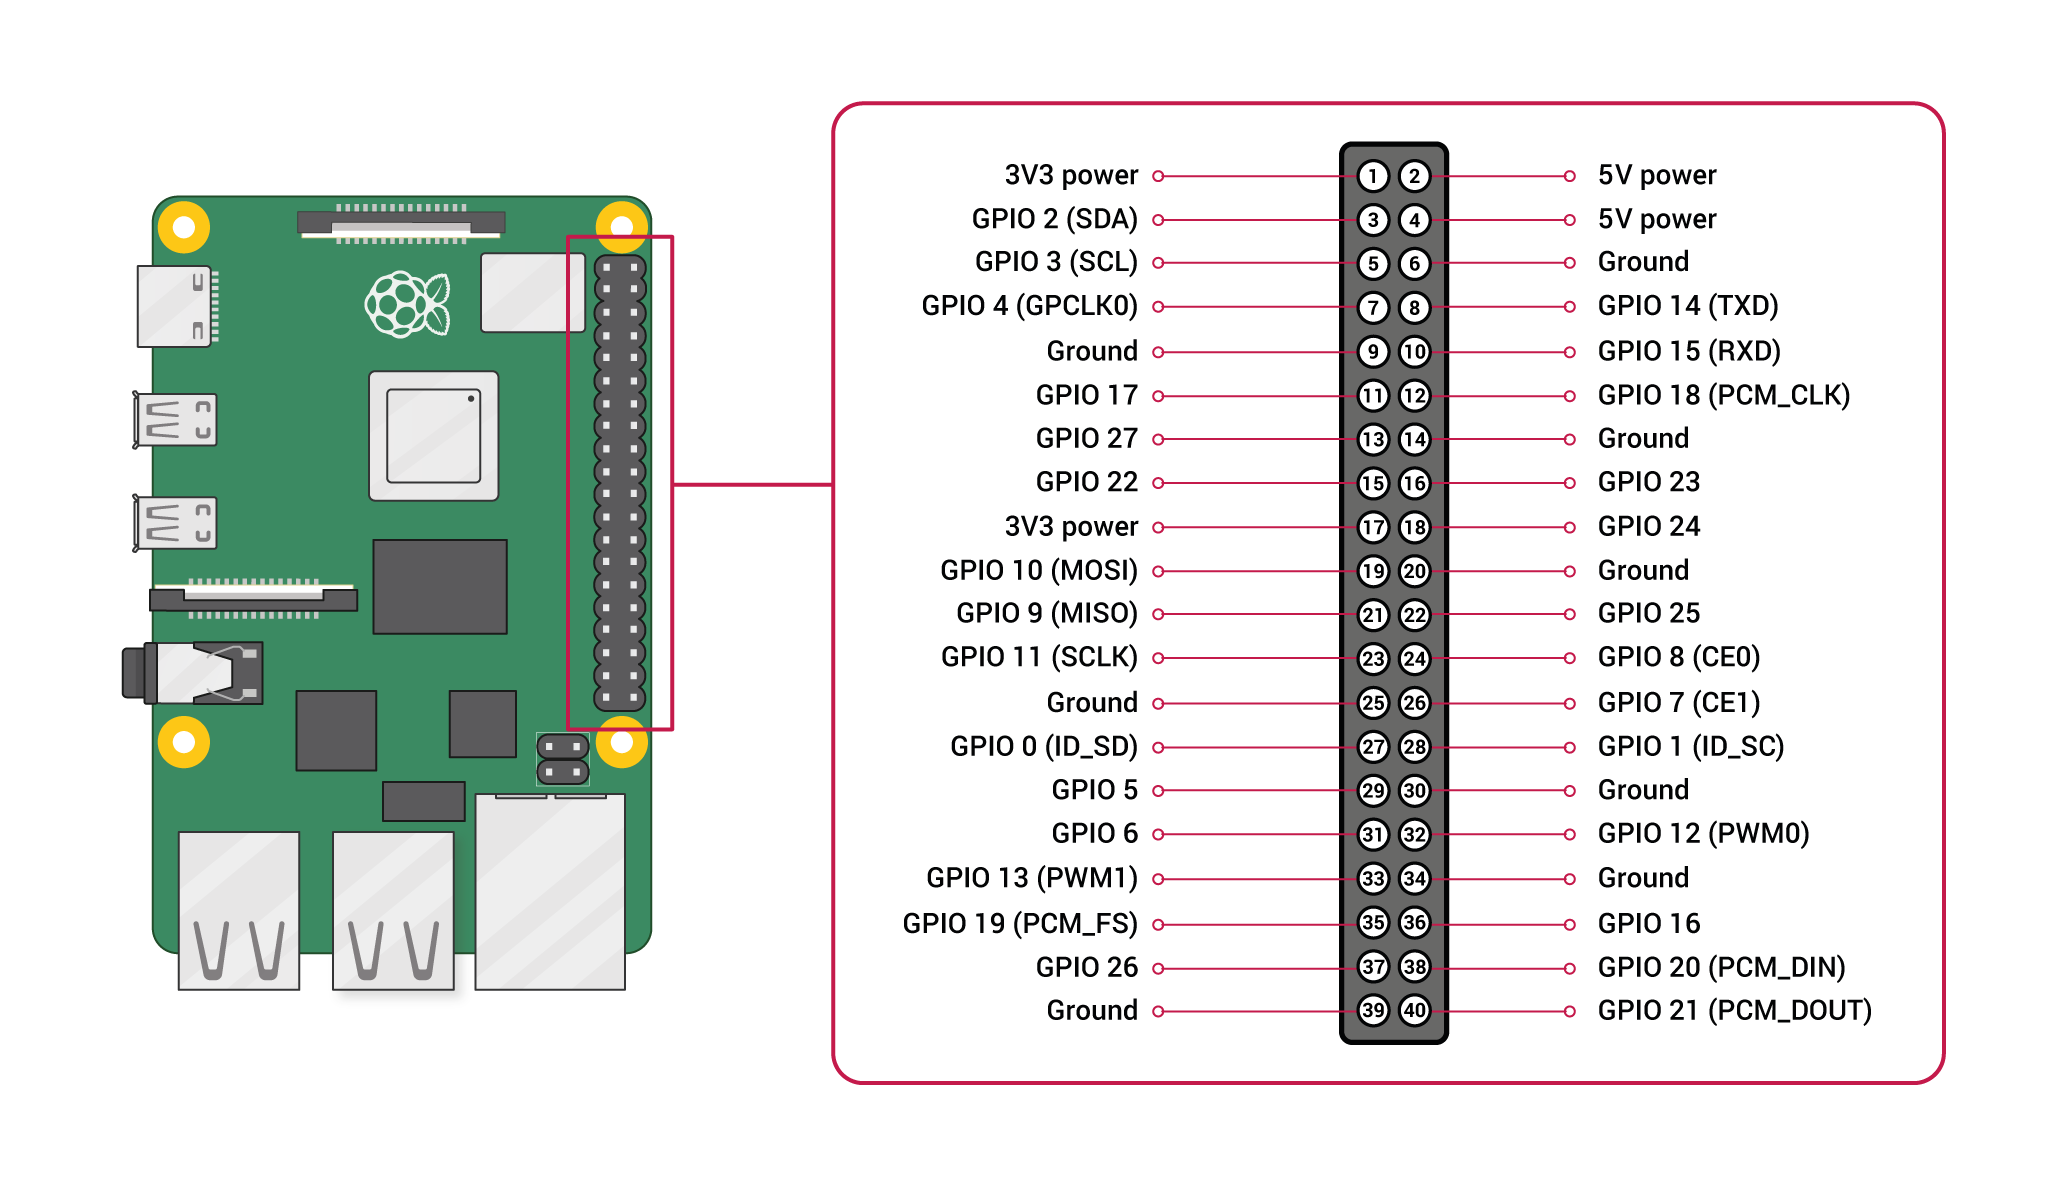
\includegraphics[width=\linewidth]{image/gpio.png} }
  \caption{A diagram showing the GPIO pins and their purposes \autocite{gpio}.}
  \label{fig:gpio}
\end{figure}

These pins are easy to interface with in software. There is a JavaScript library
that we will use for interfacing with GPIO called \url{rpi-gpio}. This library makes it
trivial to read and write data to and from these pins using simple function calls.

We will be using the GPIO pins extensively for the project for the following tasks:

\begin{itemize}
  \item Key presses
  \item Key releases
  \item Volume control
\end{itemize}

\subsubsection{Performance}

Performance is always a concern when dealing with constrained embedded hardware. The
Raspberry Pi fares better than microcontrollers you would find in a typical MIDI
controller, but is still performance constrained. Our device needs to be able to run a
machine learning model and a UI application, both of which are computationally expensive
tasks. This is a critical part of our project, so we have conducted extensive research to
ensure that what we want to do is possible on the Raspberry Pi.

\paragraph{Magenta}

Magenta serves as a good baseline for measuring performance of music generating AI.
Magenta ships with two machine learning models: MusicRNN and MusicVAE. We have performance
tested both of these in a demo benchmark program we have written on the Raspberry Pi 4B.
We have design the benchmark suites to be modular so that we can benchmark our own
checkpoints or models later in development.

The benchmark program we constructed uses Magenta with JavaScript. We use the Tensorflow
node backend for good CPU performance with Node. The program uses both the MusicRNN and
MusicVAE models, with checkpoints that are hosted are Google's servers. The checkpoints
tested are the \url{basic_rnn}, \url{melody_rnn}, and \url{drum_kit_rnn} checkpoints for
the MusicRNN, and the \url{mel_4bar_small_q2} checkpoint for \url{MusicVAE}. The benchmarks
use a JavaScript benchmarking framework called Benny to run several test cases with
magenta, sampling each one several times and providing statistics such as the min, max,
and mean generation time, as well as the standard deviation.

Our benchmarking program has two benchmarking suites: a generalized one to gauge overall
performance (see \nameref{appendix:magenta_benchmark}) and a linear suite to find out what
factors affect performance the most.

In the generalized suite, the MusicRNN model with the provided pretrained checkpoints has
shown good performance overall when autofilling simple and random melodies, well below the
5-second threshold in general with a few edge cases that exceed 5 seconds. With this
knowledge we know it is feasible to run a music generating AI on the Raspberry Pi 4B. What
we need to know is how much we are able to push the music generating AI before we fall
below our threshold. This is where the linear benchmarks come in.

The linear benchmarks allow us to figure out what constraints we have to limit ourselves
to in order to stay below our 5 second threshold. We based these benchmarks around factors
we speculated would affect the performance the most. For each of these benchmark factors,
we progressively test higher amounts and graph the results for easy analysis (see
\autoref{fig:magentaperf}).

\paragraph{Linear benchmark factors}
\begin{itemize}
  \item \textbf{Melody duration.} This is the duration of the input melody in seconds.
  \item \textbf{Number of notes.} Total number of notes in the input melody. This is with
        a constant duration of 16 seconds.
  \item \textbf{Generation steps.} Each generation step represents a quarter note in these
        benchmarks. The duration is constant at 16 seconds.
  \item \textbf{Temperature} This is the temperature of the RNN, which affects the
        randomness of the generated melodies.
\end{itemize}

All benchmarks in the linear suite use random notes quantized to quarter steps. The random
notes fit the checkpoints supported note rage, which is different between checkpoints. For
example, the \url{basic_rnn} checkpoint supports pitches in the range \url{[48, 84]},
while \url{melody_rnn} supports the full MIDI range of \url{[0, 127]}
\autocite{modelPitchRange}.

With this data collected, it becomes easy to analyze what constraints we are working
with. Our target is to remain below 5 seconds of generation time, so we need to ensure
that we have a safe margin below where the graphs meet 5 seconds. The generation time
increases linearly with melody duration and total generation steps. The \url{basic_rnn}
and \url{melody_rnn} checkpoints were neck and neck in terms of generation time, while the
\url{drum_kit_rnn} checkpoint was consistently slower. The temperature had no effect on
the generation time. We were initially surprised to see that the total number of notes had
no effect on generation time, which remained constant when increasing from 100 to 2000
input notes, but this makes sense as the input tensor size does not change with the number
of notes.

The input duration is the biggest factor affecting generation time. The number of
generation steps are the next biggest factor. With this data, we know that we will most
likely need to truncate the input melody's duration to less than 40 seconds of music. The
generation steps need to be accounted for when determining the duration of music to accept
as input for our AI. As the generation steps increase we need make up for that amount of
extra time by decreasing the input duration even further. We added in a benchmark for
increasing duration and generation steps simultaneously to see if this would lead to
exponential behavior, but found that it remained linear. So we can simply subtract the
estimated added time from the input melody duration.

With these benchmark results, we are confident that the Raspberry Pi 4B is capable of
handling the computational load that this project requires, without the need for any
external processing. We also have a good benchmarking solution that can be adapted for any
checkpoints or models that we will further into the project's development.

\begin{figure}
  \centerline{ 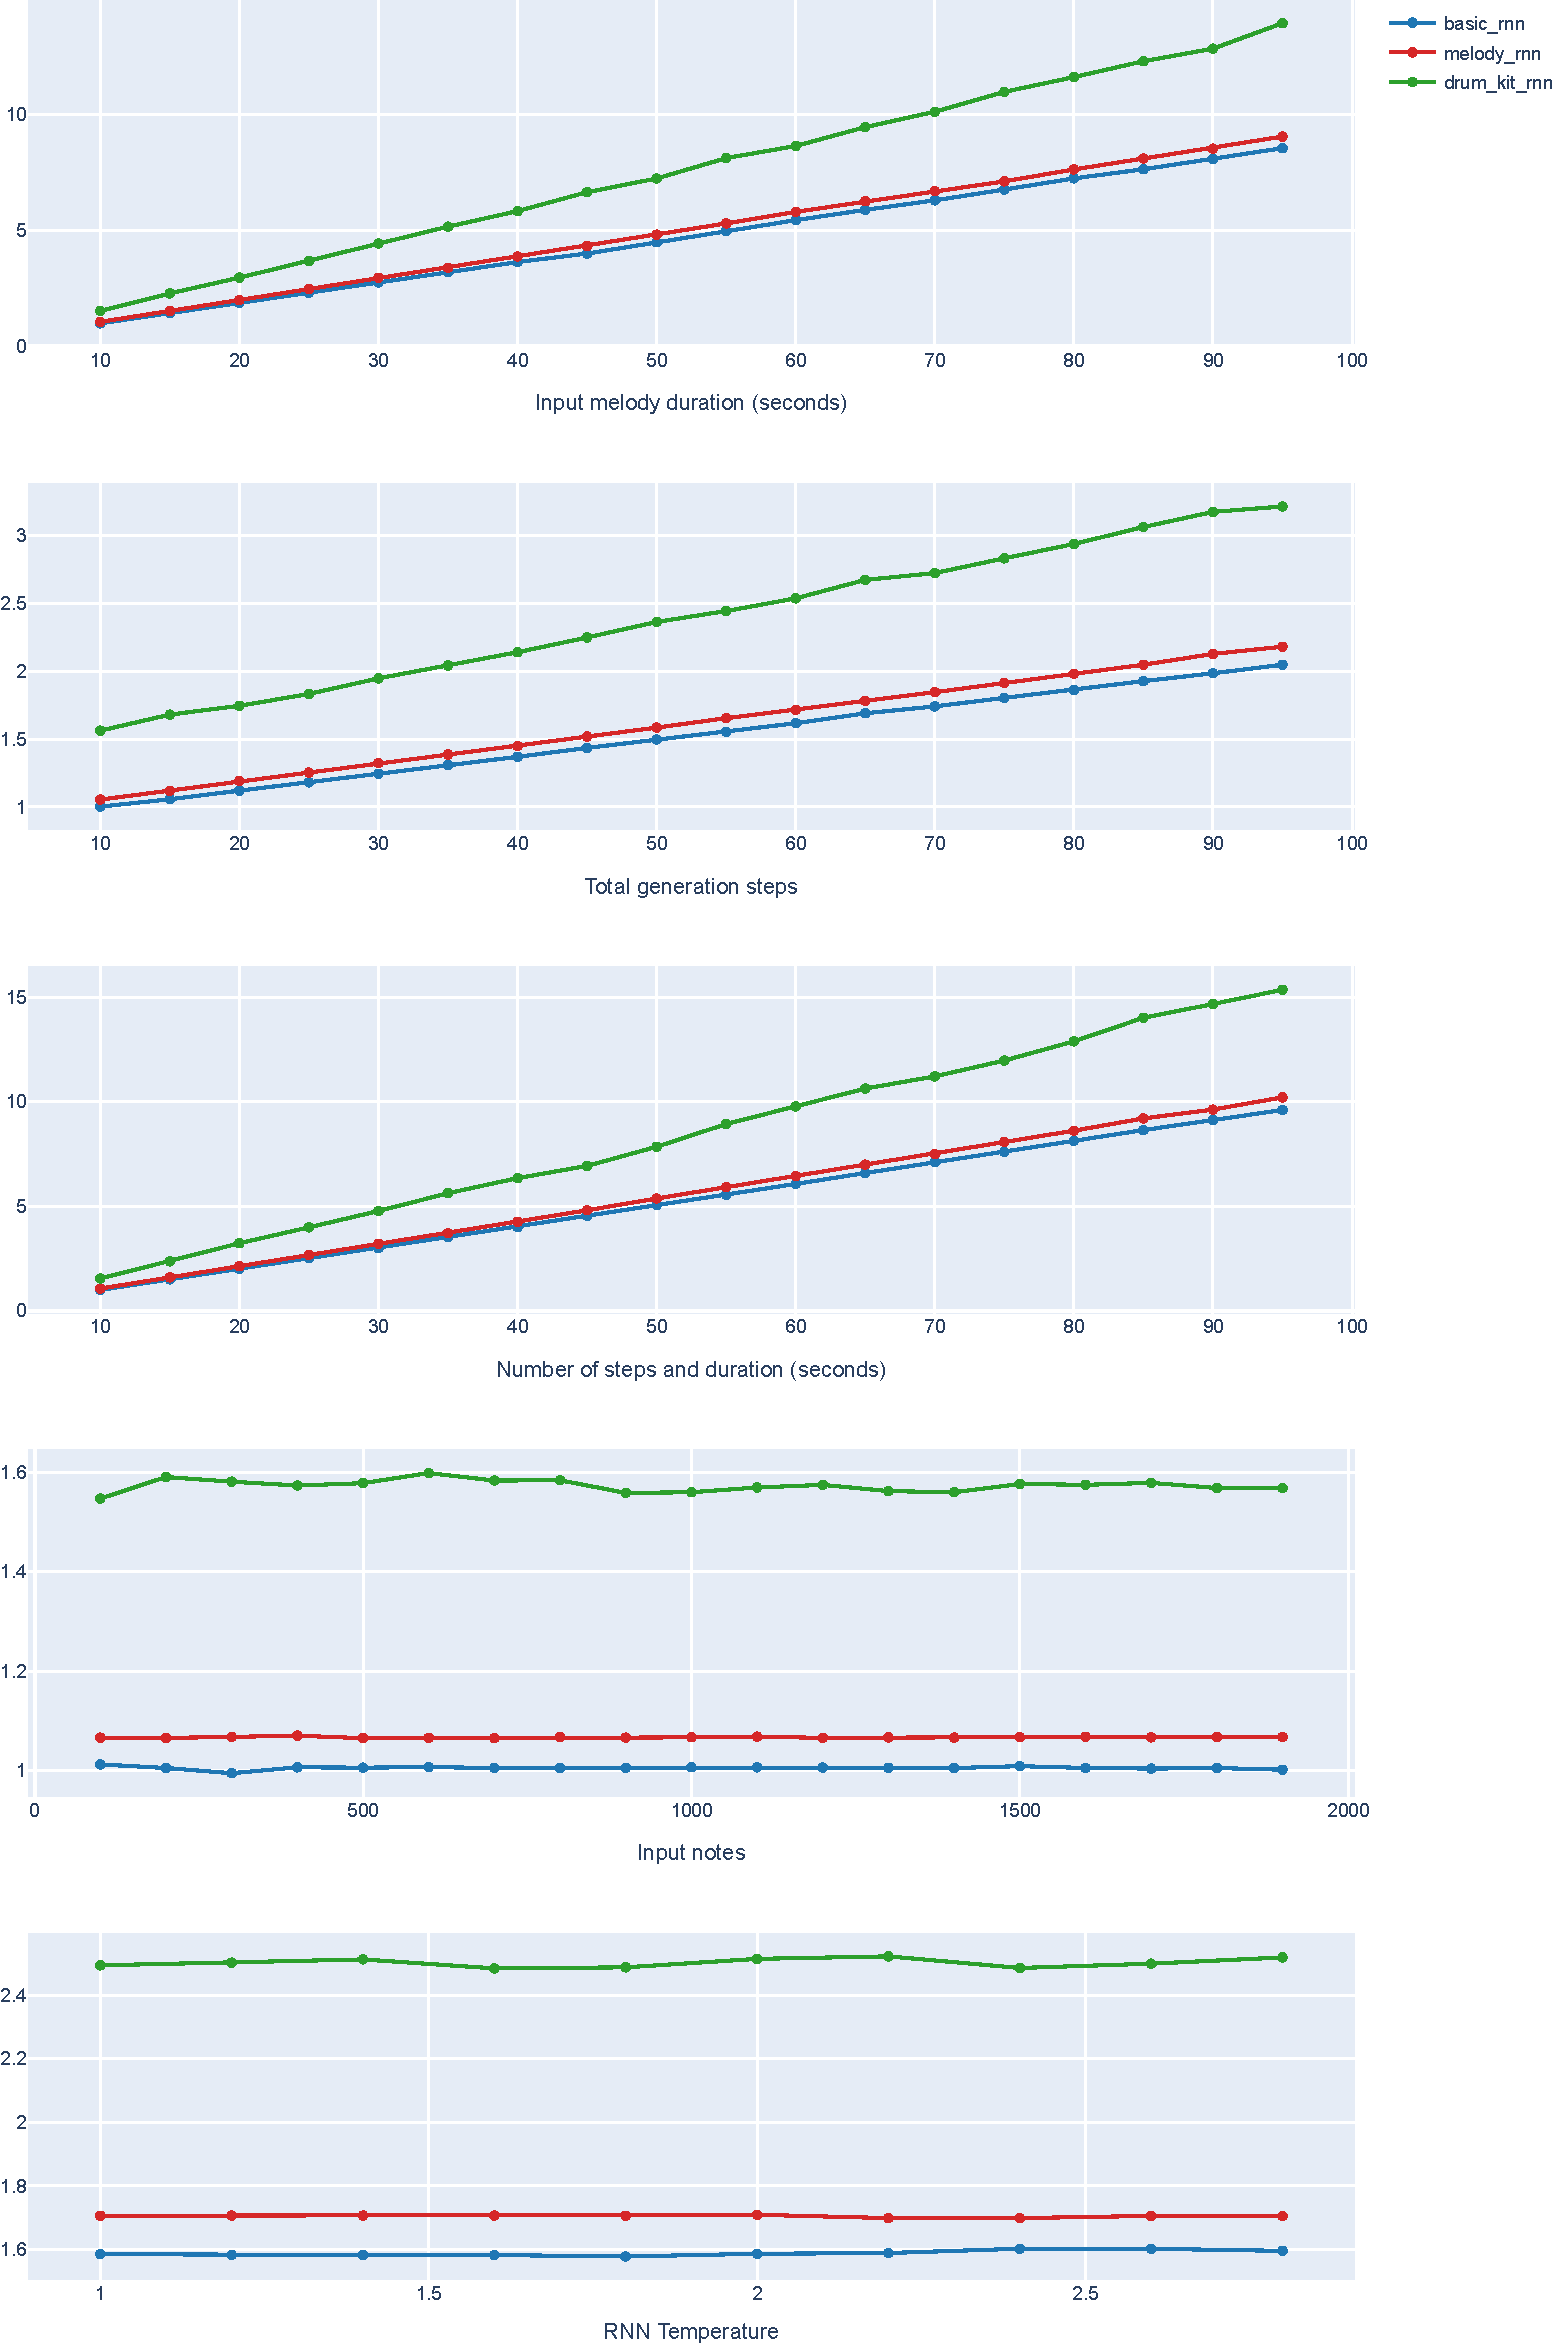
\includegraphics[width=.95\linewidth]{image/perf.pdf} }
  \caption{Magenta Generation Time on the Raspberry Pi 4B.}
  \label{fig:magentaperf}
\end{figure}

\paragraph{UI.} It is important to verify that a Raspberry Pi can even run a browser based
DAW with acceptable performance before spending development time creating the web app.
Since we have not developed the DAW at this point, we have tested an existing web based
MIDI editor in the Raspberry Pi.

We used an online MIDI editor called signal (\url{https://signal.vercel.app/}) to get a
subjective feel for the performance. The test was run in the chromium web browser on
Raspberry Pi OS. The performance was acceptable, with some actions feeling slow.
Dragging around notes had a small but noticeable latency between the mouse cursor's
movement and the notes position. There was also a small but noticeable latency between
double clicking to insert a note and the note showing up on screen. The playhead updated
smoothly when playing the MIDI track, which is the most important aspect, as laggy
playback is awful for the user experience.

It should be noted that this app was not explicitly designed to run on constrained
hardware. Web apps can run great on Raspberry Pis when optimized to do so. Based on our
findings here we are confident that we can develop a browser based app that has
exceptional performance on the Raspberry Pi.

\subsection{MIDI Peripheral}
\label{sec:midi_peripheral}

The Pi needs to function as a MIDI peripheral, with the user being able to connect the
device into a computer and have it function as a device that sends MIDI commands to the
DAW. There are a few different ways to approach this connection, and we have explored a
few such approaches for this project.


\subsubsection{USB-C Connection}

Under this approach, the connection will happen through a USB-C to USB-A cable from the
Raspberry Pi to the computer. The Raspberry Pi is typically powered from the USB-C port
form a power supply connected to a power outlet, but in our case the Pi will receive its
power from the host PC over USB-C instead. Once plugged in, the Pi will act as a normal
MIDI peripheral, which sends MIDI events to the PC, which can be picked up by a fully
fledged DAW.

The MIDI communication happens over USB in our case, which means we need to work with the
operating system to send these messages. We are using Linux for our device's operating
system, so USB communication needs to happen through the Linux kernel. This is known as a
USB Gadget in the Linux kernel \autocite{usbGadgetDocumentation}. The Raspberry Pi 4b can
act as a Linux USB Gadget through a USB-C to USB-A connection to the computer, with USB-C
being on the Raspberry Pi and USB-A being on the host computer
\autocite{raspberryPiGadgetSetup}. This will not work out of the box, as the Linux kernel
needs to be made aware that we intend to use the device as a USB gadget. This
configuration happens through files in the \url{/boot/} directory
(see listings \ref{lst:bootconfig} and
\ref{lst:bootcmdline}) \autocite{raspberryPiGadgetSetup}. The Pi will act as a USB
gadget after Linux boot configuration settings are set and it is plugged up to the host
machine.

\begin{minipage}{\linewidth}

  \begin{lstlisting}[language=bash,
  label={lst:bootconfig},
  caption=Lines added to /boot/config.txt \autocite{raspberryPiGadgetSetup, raspberryPiHDMIFix}.]
dtoverlay=dwc2
hdmi_force_hotplug=1
hdmi_group=2
hdmi_mode=87
hdmi_cvt=800 480 60 6 0 0 0
hdmi_drive=1
  \end{lstlisting}

  \begin{lstlisting}[language=bash, label={lst:bootcmdline}, caption=DietPi /boot/cmdline.txt modified to allow a USB Gadget \autocite{raspberryPiGadgetSetup}., breaklines=true]
console=ttyS0,115200 console=tty1 root=PARTUUID=8f4dbd00-02 rootfstype=ext4 elevator=deadline fsck.repair=yes rootwait quiet net.ifnames=0 modules-load=dwc2,g_ether
  \end{lstlisting}

  \begin{lstlisting}[label={lst:usb_gadget}, caption=Bash procedure to setup a MIDI Gadget\, modified for our device \autocite{raspberryPiGadgetSetup}., breaklines=true]
cd /sys/kernel/config/usb_gadget/
mkdir -p midi_over_usb
cd midi_over_usb
echo 0x17e8  > idVendor
echo 0xb09c > idProduct
echo 0x0100 > bcdDevice
echo 0x0200 > bcdUSB
mkdir -p strings/0x409
echo "fedcba9876543210" > strings/0x409/serialnumber
echo "MIDI Autofill Group" > strings/0x409/manufacturer
echo "MIDI Autofill Device" > strings/0x409/product
  \end{lstlisting}

\end{minipage}

After the boot configuration options are set, the device will be a USB gadget, but there
is more configuration needed for it to act as a MIDI USB gadget. The Linux kernel already
provides an interface for USB gadgets to act as MIDI devices, through the
\url{usb_f_midi.ko} kernel module \autocite{usbGadgetDocumentation}. We need to set our
Raspberry Pi's USB gadget settings to identify itself as a MIDI peripheral. We have
followed an online guide to setup this MIDI gadget, which involves providing information
to the kernel about our device through the \url{/sys/kernel/config/usb_gadget/} folder
\autocite{raspberryPiGadgetSetup}.

From here we can use the \url{aplaymidi} command to test our MIDI device, which sends a
MIDI file to the host computer \autocite{gadgetTesting}. If the gadget is working
properly, then the MIDI sequences should be visible in any application that listens for
MIDI note events, such as a DAW.

USB Gadgets appear as USB ethernet devices and can be read and written to like any other
networking interface. USB MIDI gadgets similarly communicate through standard networking
interfaces under Linux, meaning that our backend program for sending MIDI events to the
host computer will be sending messages through networking interfaces. However, we will
most likely use a library to abstract away this networking aspect.

USB gadgets work, but we ran into a problem with our setup where our HDMI connection to
the monitor was not working anymore. This connection is critical, as we need to be able to
display our DAW to the built in connection using HDMI, so we had to find a workaround for
this issue. We found out that there are \url{/boot/config.txt} options that can added to
force an HDMI connection, using the \url{hdmi_force_hotplug} option
\autocite{raspberryPiHDMIFix}. This configuration as well as some other HDMI settings can
be seen in listing \ref{lst:bootconfig}.

We have also run into some low voltage warnings when running the Raspberry Pi 4B as a USB
gadget. These warnings are found in system logs and are viewed with \url{journalctl}. The
Raspberry Pi 4b requires 5.1 volts and 3 amps to operate effectively, and will send the
undervolt warning whenever it runs below 4.63 volts \autocite{raspberryPiAmps}. We notice
that we see these warnings early in the boot, but it seems to stabilize later. We have not
run into any issues with these undervolts as of now. The Pi does not encounter anymore
voltage warnings when running a CPU stress test, but it could lead to stability issues
later.

This approach was our preference, but we ran into a wall when considering how to allow the
device to function as a standalone device, while also being able to receive power through
the USB-C connection. USB gadgets are supposed to be powered through the USB-C port, but
when not connected, the USB device will operate off of a battery. The standalone operation
requirement makes this connection mode very difficult. There is another interface for
powering the raspberry PI, which is the 5 volt GPIO pin. This could be connected to a
battery. But then there is the question of if the Pi can be simultaneously powered by the
5 volt GPIO port while also being plugged in with USB-C. This may be possible, but there
are no resources online that show how this can be done. It is not worth the time to figure
out how this can be done.

\paragraph{Pros}

\begin{itemize}
  \item Lowest latency
  \item Simplest setup, only requiring the end-user to plug in the device
\end{itemize}

\paragraph{Cons}

\begin{itemize}
  \item Wired
  \item Implementation is too complex
\end{itemize}

\subsubsection{RTP-MIDI Over WIFI}

RTP-MIDI is an open source protocol to send and receive MIDI messages over standard
networking interfaces. RTP-MIDI is built over Real-time Transport Protocol (RTP), which is
a protocol for real-time communication over the network. RTP typically works through UDP
messages over IP. RTP-MIDI can be used over a LAN network. When used over WIFI, the MIDI
device can be connected to another computer without a wired connection. This wireless
factor is convenient for the end user.

With wireless connections, there is always a question of if it can achieve acceptable
latencies. RTP-MIDI over WIFI is fast, and latency is not a major concern. RTP-MIDI Over
WIFI has a latency of around 8.5 ms with a standard deviation of 8 ms
\autocite{ble-latency}.

A major disadvantage of RTP-MIDI is that it is not supported out of the box in Windows 10.
Since RTP-MIDI are just simple UDP network messages, this can be worked around by
downloading a driver, or by using a standalone piece of software. Requiring the user to
download extra software to the computer will degrade the user experience. We want the user
to be able to use the MIDI device with minimal extra setup, and this would hamper that
experience. Addtionally, the user would need to know the IP address of the device on the
LAN, and enter it into the software. This is another step that will hamper the out of box
experience. This can be avoided if the user is running the Bonjour service, but that is
another step that could potentially cause problems.

This approach would be the easiest to implement from a developer perspective. These are
just simple network messages, without the need to go through any special interfaces. There
is a NodeJS library called \url{node-rtpmidi} which would make RTP-MIDI trivial to
implement on the Raspberry Pi. It would be a matter of simply making the connection and
using the library to send MIDI messages.

\paragraph{Pros}

\begin{itemize}
  \item Wireless
  \item Simplest implementation
  \item Lower latency than the Bluetooth solution
\end{itemize}

\paragraph{Cons}

\begin{itemize}
  \item Higher latency than USB
  \item Requires the user to download additional software
  \item Most difficult for the end-user to setup
\end{itemize}

\subsubsection{MIDI Over Bluetooth Low Energy}
\label{sec:ble_midi}

Bluetooth Low Energy (BLE) is a wireless technology standard that enables BLE compatible
devices to communicate with one another. Despite the namesake, BLE is separate from
classic Bluetooth, intended to consume less power, and is not backwards compatible with
classic Bluetooth. Common examples of BLE devices include BLE speakers, keyboards and
mice. The Raspberry Pi 4B supports BLE, which means that the Raspberry Pi can act as a BLE
device. Using BLE has the benefit of being convenient for the end-user as well, with the
ability to move the device freely and without needing to manage another cable.

Most computers also support BLE, or can be made to support BLE through the use of a
Bluetooth USB Dongle. While BLE is not as prevalent as USB, compatibility should not be a
concern for the majority of devices. Bluetooth is also easy for the end-user to setup,
only requiring the end-user to connect to the device through the operating system's
interface.

BLE can be used for a wide variety of devices. BLE devices communicate through profiles,
which specify the BLE  application and the communication specifications. There is a long
list of standardized BLE profiles, with one such profile being BLE MIDI. While support for
BLE is very common, support for certain BLE profiles is not, as its up to each BLE
implementation to support whatever profiles are needed by the device. However, BLE MIDI is
supported by Windows 10, MacOS, Linux, iOS, and Android \autocite{ble-latency}. With BLE
MIDI being supported by every major operating system, we are confident that we will not
run into any compatibility issues with this approach, except for on older computers.

We initially thought that using BLE would incur too much input latency to be practical for
musicians. Using Bluetooth audio is notorious for its latency. But the latency situation
with BLE MIDI is much better than Bluetooth audio. BLE MIDI has higher latency than USB
MIDI, but the numbers are acceptable. BLE MIDI events have a delay of approximately 12
milliseconds one-way and 26ms round-trip time \autocite{ble-latency}. We find this
latency number to be acceptable for our project.

The Raspberry Pi runs Linux, which means that it needs to work through the BlueZ stack in
order to function as a BLE device. BlueZ is a component of Linux that implements Bluetooth
and BLE. The BlueZ stack supports MIDI over BLE, and in combination with ALSA, it is
possible to turn a Raspberry Pi into a BLE MIDI device.

Audio under Linux is handled through the ALSA interface. ALSA also provides what are known
as sequencer ports, which are used to send MIDI events through an interface that can be
connected to a variety of targets. In combination with BlueZ, we can create an ALSA
sequencer port to send MIDI events over BLE. BlueZ provides a binary called
\url{bt-midi-server}, which creates an ALSA sequencer port that is connected to a BLE MIDI
output. From there, we can send MIDI events over BLE by simply using the ALSA APIs for
sequencer ports. When \url{bt-midi-server} is started, any MIDI Bluetooth connections will
automatically get connected to an ALSA sequencer port. This is a nice abstraction which
allows us to write MIDI code without needing to consider Bluetooth in the code itself. The
\url{bt-midi-server} can be run at startup using a systemd service. Our code will simply
need to check for the existence of the sequencer port to see if we're connected to
Bluetooth.

ALSA sequences are programmed using a C API. This C API can be called from JavaScript
using the Foreign Function Interface (FFI). In this API, clients send sequencer events
through the port, which can encode various MIDI events, such as note on/off, with data
such as the pitch and velocity. This API is simple to use, and will be easy to integrate
into our application.

With this interface, it is easy to create a program that creates a ALSA connection to the
BLE MIDI sequencer port, listens for the key presses from GPIO events, interprets those
GPIO events, and sends the corresponding MIDI commands to the ALSA sequencer port. The BLE
connection is abstracted away in this configuration, allowing us to just focus on writing
MIDI code.

\paragraph{Pros}

\begin{itemize}
  \item Wireless
  \item Widely supported by all operating systems
  \item Simple implementation
\end{itemize}

\paragraph{Cons}

\begin{itemize}
  \item Highest latency
  \item Extra connection step required from the end-user
\end{itemize}

\subsubsection{Conclusion}

We have decided to go with the MIDI over Bluetooth Low Energy approach. This approach does
to suffer from the same problems the USB-C approach has, and provides an added convenience
factor, allowing the user to use the device without wires. It is also easier for the
end-user to configure, with the end-user only needing to connect to a Bluetooth device
through the operating system's Bluetooth interface. The latency is higher than USB-C, but
it is within our specifications. The implementation is also simpler than using USB-C.

\subsection{Application Architecture}
\label{sec:app_architecture}

Our application will be composed of components that will need to interact with each other.
These components are the UI, music generator, and the MIDI device interface. These
components individually are more suited to be programmed in different languages and
environments, which makes it important to consider how these components should be
designed. There are a few different approaches to the application architecture that have
their own pros and cons. The possibilities we have considered are monolithic application,
a multi-process approach, and a library approach.

\subsubsection{Monolithic Architecture}

This is the simplest approach with a single program handles all aspects of the
application. This single application will display the DAW UI, generate the notes, and act
as the MIDI device interface. Everything would be a single project, and there would not be
a need for any inter-process communication (IPC).

The main advantage here is architectural simplicity. Having separate components makes the
project harder for developers to grasp. Generally, it is easiest to develop a single
application where feasible.

Another advantage is simpler maintenance. With a multi-process approach, when one
component changes, often it is necessary to update other components to work with these
changes.

The main problem with this approach is that some components are done better in other
languages and with different environments. For our UI, we are going for a web-based
approach, which would mean using a NodeJS stack. We can generate the notes using
JavaScript as well, as there is Tensorflow for JavaScript. But tensorflow is mainly
intended to be used with python, and there is an ecosystem of AI tools and documentation
we will miss out on when using JavaScript, which will make the implementation more
difficult than python. Futhermore acting as a MIDI device is a low-level process that is
best implemented with a low-level language such as C. Like before, in this instance its
possible to be done in a NodeJS ecosystem, but not ideally.

\paragraph{Pros}

\begin{itemize}
  \item Architecturally simple
  \item No need to implement IPC
  \item Ease of deployment
\end{itemize}

\paragraph{Cons}

\begin{itemize}
  \item Difficulty implementing certain components
  \item Errors affect the whole application
  \item Easy to create highly coupled designs
\end{itemize}

\subsubsection{Multi-process Architecture}

In a multi-process architecture, each major component will run in its own executable, and
communicate using an IPC mechanism. Each component can be developed in an ideal ecosystem,
with the UI being a web-based JavaScript application, the music generator being a python
component, and the MIDI device interface being a low-level C component.

Since these components are not in a single executable, they all need to run concurrently,
which means there will need to be a mechanism that spawns all processes. There are a
number of ways to spawn all these processes, such as using system services, or having a
main process that spawns all the child processes and negotiates the IPC mechanism to all
children. For simplicity, here we are mainly considering the main process approach.

An essential part of this is the IPC mechanism, and there many ways to handle IPC. One
mechanism is to start TCP server over localhost. Components can know where to communicate
based off the port number. This communication mechanism allows for any format of
communication in the body, such as JSON. There are two downsides to this IPC approach. The
first downside is the overhead of having to go through the networking systems of the
operating system. The second downside is the potential of port conflicts, if another
application wants to use a port we designate, but this should not be a problem for our
case as our operating system configuration is tailored to our application. Another
approach we consider is to use Unix domain sockets, which works over networking interfaces
(sockets), but works over a file instead of ports. This approach has less overhead and
doesn't have a port conflict issue. The downside here is more implementation complexity,
as there are fewer libraries and resources for communicating over domain sockets instead of
TCP. If we intended to go with this architecture, this is the IPC mechanism we would
choose.

The IPC mechanism will require additional code, which will slow development time and
create another maintenance hassle. Not only will there need to be code for using Unix
domain sockets, but there will also need to be code to parse and interpret the messages.
The message format will need to be designed and standardized between the applications, and
if any messages need to change, those changes will need to be reflected in all the
components. For example, if JSON is used for the messages, then any time a field changes,
or another field is added, components that use that message will need to be updated to
interpret the new data structure. Parsing JSON is trivial in python and JSON using third
party dependencies, but doing so in C, which the MIDI interface component would be
programmed in, would be difficult, even with third party libraries. Even in python and
JavaScript, which parse JSON trivially, there is still work to agree on a format.

As mentioned earlier, the main advantage to this approach is to be able to create
components in their ideal language and environments. This is a big advantage for the AI in
particular, as python is the most common choice to develop machine learning AI in, and
there are more libraries, documentation, and tutorials to develop machine learning
applications in python.

\begin{figure}[h!]
  \centering
  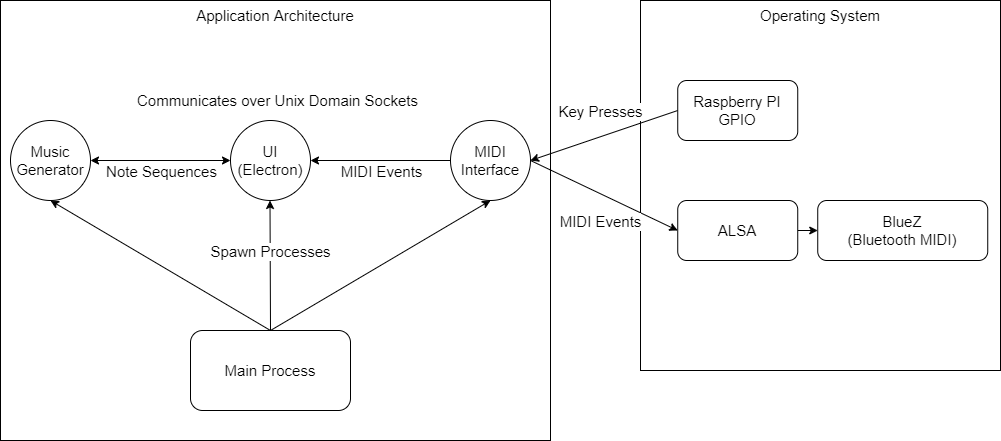
\includegraphics[width=\linewidth]{image/multiprocess.png}
  \caption{Proposed Multi-process Architecture.}
  \label{fig:multiprocess}
\end{figure}

\paragraph{Pros}

\begin{itemize}
  \item Ideal language and environment for all components
  \item Loosely coupled design
\end{itemize}

\paragraph{Cons}

\begin{itemize}
  \item Architectural complexity
  \item Need to implement IPC
  \item Need to manage child processes
  \item Need to create a messaging format and parse that format in all processes
\end{itemize}

\subsubsection{Library Approach}

In this approach, there is a main executable supplemented by libraries. The main process
will be a NodeJS based web application and it would libraries for the Music Generation and
MIDI device interface will be handled by external libraries. This would allow the
components to be developed in different languages and environments without the need to
implement IPC and child process management. This approach seemed ideal initially, but
there are some caveats that make this infeasible. Creating a library requires the
developer to create bindings to the libraries. Different languages have different binary
interfaces. The Application binary interfaces (ABI) defines how functions and data
structures are laid out in memory. Bindings are used to bridge the differences between the
ABIs of both languages to allow a library written in one language to be used in another
language.

For the MIDI device interface, which will be programmed in C, this approach works well.
Both JavaScript and Python can call C code through a foreign function interface (FFI). C
has the closest to what can be considered a standard ABI, with the SystemV ABI being a
standard in Linux, with all binaries being in the standard Executable and Linkable Format
(ELF) format. Using the \url{node-ffi} library in NodeJS, the main JavaScript process can
easily integrate with a C library. It is not as straightforward as using a normal
JavaScript library, but it does not take much effort. Python can also interface with C
libraries through its built in CFFI module, but that will not be necessary for this
project.

Where this approach falls apart is creating a binding to python for the music generation
component. Python is an interpreted language, meaning that it is evaluated at runtime
rather than precompiled to a binary. To use python in another language, rather than using
a traditional library, python must be embedded into other languages. Embedding allows a
program written in another language to have parts implemented in a scripting language.
Python provides a C library for embedding python code. This is commonly used in games, for
example, where the bulk of the game is implemented in C++ and then simpler tasks are
implemented in a high-level language such as Python for developer productivity. This would
work, but would be tedious in a C or C++ application. In our case, we would need it to be
embedded in a NodeJS application, which is even more tedious. There is a Node library
called \url{pynode} to assist in this process, but it would still cost too much
development time.

\paragraph{Pros}

\begin{itemize}
  \item Ideal language and environment for all components
  \item Loosely coupled design
  \item No need to implement IPC
  \item No need to implement child processes
\end{itemize}

\paragraph{Cons}

\begin{itemize}
  \item Need to implement FFI code
  \item Need to implement code to embed python in Node, which is not straightforward
\end{itemize}

\begin{minipage}{\linewidth}

  \begin{lstlisting}[language=JavaScript, label={lst:node_ffi}, caption=Example of using \url{node-ffi} to call a C library \autocite{node-ffi}., breaklines=true]
var ffi = require('ffi');

var libm = ffi.Library('libm', {
  'ceil': [ 'double', [ 'double' ] ]
});
libm.ceil(1.5); // 2

// You can also access just functions in the current process by passing a null
var current = ffi.Library(null, {
  'atoi': [ 'int', [ 'string' ] ]
});
current.atoi('1234'); // 1234
\end{lstlisting}

\end{minipage}

\begin{minipage}{\linewidth}

  \begin{lstlisting}[language=Python, label={lst:pynode}, caption=Example of using \url{pynode} to embed python in JavaScript \autocite{pynode}., breaklines=true]
const pynode = require('@fridgerator/pynode')

// Workaround for linking issue in linux:
// https://bugs.python.org/issue4434
// if you get: `undefined symbol: PyExc_ValueError` or `undefined symbol: PyExc_SystemError`
pynode.dlOpen('libpython3.6m.so') // your libpython shared library

// optionally pass a path to use as Python module search path
pynode.startInterpreter()

// add current path as Python module search path, so it finds our test.py
pynode.appendSysPath('./')

// open the python file (module)
pynode.openFile('example')

// call the python function and get a return value
pynode.call('add', 1, 2, (err, result) => {
  if (err) return console.log('error : ', err)
  result === 3 // true
})
\end{lstlisting}

\end{minipage}

\subsubsection{Conclusion}

We have decided to go with the monolithic application approach. While it makes more sense
for the AI to be programmed in JavaScript and the MIDI interface to be programmed in C, it
is not worth the extra development effort to have to deal with IPC or FFI/embedding code.
The application will be a single NodeJS application for displaying the UI, generating the
notes, and creating an interface as a MIDI device. JavaScript can still use TensorFlow
through the TensorFlowJS binding. There are JavaScript libraries for dealing with MIDI,
and the FFI can also be used for any other functionality that is needed for MIDI interface
support.
